\documentclass[12pt]{article}
\usepackage[a4paper,left=2.5cm,right=2.5cm,top=2.5cm,bottom=2.5cm]{geometry}
%\usepackage[margin=0.5in]{geometry}
\usepackage[utf8]{inputenc}
\usepackage{graphicx}
\usepackage{float}
\usepackage{multicol}
\usepackage{wrapfig}
\usepackage{multirow}
\usepackage{subcaption}
\graphicspath{ {./images/} }
\usepackage{amssymb}
\usepackage{amsmath}
\usepackage{graphicx}
\usepackage{epstopdf}
\usepackage{bm}
\usepackage{mdframed}

\usepackage{cite}

%\usepackage[
%backend=biber,
%style=authoryear,
%sorting=ynt
%]{biblatex}
%\addbibresource{project_log.bib}


\usepackage{hyperref}
\hypersetup{
    colorlinks=true,
    linkcolor=blue,
    filecolor=magenta,      
    urlcolor=cyan,
}
%\urlstyle{same}


\usepackage{listings}
\usepackage{xcolor}
\definecolor{codegreen}{rgb}{0,0.6,0}
\definecolor{codegray}{rgb}{0.5,0.5,0.5}
\definecolor{codepurple}{rgb}{0.58,0,0.82}
\definecolor{backcolour}{rgb}{0.95,0.95,0.92}

\lstdefinestyle{mystyle}{
	backgroundcolor=\color{backcolour},   
	commentstyle=\color{codegreen},
	keywordstyle=\color{magenta},
	numberstyle=\tiny\color{codegray},
	stringstyle=\color{codepurple},
	basicstyle=\ttfamily\small,
	breakatwhitespace=false,         
	breaklines=true,                 
	captionpos=b,                    
	keepspaces=true,                 
	numbers=left,                    
	numbersep=5pt,                  
	showspaces=false,                
	showstringspaces=false,
	showtabs=false,                  
	tabsize=2
}
\lstset{style=mystyle}


\newcommand{\bma}{\begin{math}}
\newcommand{\ema}{\end{math}}
\newcommand{\beq}{\begin{equation}}
\newcommand{\eeq}{\end{equation}}
\newcommand{\beqa}{\begin{eqnarray}}
\newcommand{\eeqa}{\end{eqnarray}}
\newcommand{\beqal}{\begin{aligned}}
\newcommand{\eeqal}{\end{aligned}}
\newcommand{\bc}{\begin{center}}
\newcommand{\ec}{\end{center}}
\newcommand{\bit}{\begin{itemize}}
\newcommand{\eit}{\end{itemize}}


\def\n{{\bf  \hat n}}
\def\k{{\bf k}}
\def\l{{\bf l}}
\def\L{{\bf L}}
\def\r{{\bf r}}
\def\x{{\bf x}}
\def\u{{\bf u}}
\def\F{{\bf F}}
\def\K{{\rm K}}
\def\mK{{\rm mK}}
\def\arcmin{{\rm arcmin}}
\def\ln{{\rm ln}}
\def\max{{\rm max}}
\def\min{{\rm min}}
\def\tot{{\rm tot}}
\def\iul{{\rm I}}
\def\il{{\tilde{\rm I}}}
\def\itot{{\tilde{\rm I}^{\rm tot}}}
\def\pul{{\rm P}}
\def\pl{{\tilde{\rm P}}}
\def\ptot{{\tilde{\rm P}^{\rm tot}}}
\def\cul{{\rm C}}
\def\cl{{\tilde{\rm C}}}
\def\ctot{{\tilde{\rm C}^{\rm tot}}}
\def\km{{\rm km}}
\def\kg{{\rm kg}}
\def\h{{\rm h}}
\def\erf{{\rm erf}}
\def\erfc{{\rm erfc}}
\def\mpch{{\rm Mpc/h}}
\def\mhz{{\rm MHz}}
\def\d2l{\frac{d^2l}{(2\pi)^2}}
\def\dko{\frac{dk_1}{2\pi}}
\def\dkt{\frac{dk_2}{2\pi}}
\def\dtheta{\delta \theta}
\def\dang{\mathcal{D}}



\numberwithin{equation}{section}
\begin{document}
\tableofcontents
\pagebreak

\section{Extending Hu's quadratic estimator to three dimensions}
\paragraph{Objective} To understand eq. 22 to 31 in Zahn and Zaldarriaga 2006

\subsection{Introduction}
\begin{itemize}
	\item Unlike CMB, we can use information from multiple planes in the case of 21 cm signal.
	\item But the different planes would be correlated. No simple way to take this correlation into account while constructing the estimator.
	\item Instead, we divide the 3D temperature fluctuations into radial and transverse parts.
\end{itemize}

\subsection{Notation}
We use the terminology and notation as described in \href{http://arxiv.org/abs/astro-ph/9905116v4}{Hogg 2000 arXiv:9905116}.
\paragraph{Observed volume}
\begin{itemize}
	\item We define the observed volume as
		\begin{itemize}
			\item located at redshift $ z $. 
			\item having a width of solid angle $ d\Omega $ along the transverse direction as seen by the observer
			\item having the depth along the line of sight $ \mathcal{L} $ = comoving distance between redshift $ z$ and $ z' $, where $ z < z' $ ($ D_C $ in Hogg 2000).
		\end{itemize}
	\item The  distance between the observer and the volume is $ \chi $. It is called transverse comoving distance as per the definition in Hogg 2000 ($ D_M$ in this paper).
	\item The transverse comoving size of the volume is $ S $. 
\end{itemize}

\paragraph{Intensity field}
Field $ I(\textbf{x}) $ at position $ \textbf{x} $ in comoving space
\beq
\beqal
I(\textbf{r}) &= \int \frac{d^3\k}{(2\pi)^3} \il(\k) e^{i \k \cdot \x}
\\
&= \int \frac{d^2\l}{(2\pi)^2} \int \frac{dk_{\parallel}}{2\pi} \frac{\il(k_\perp, k_\parallel)}{\chi^2} e^{i(\l\cdot \theta + k_\parallel x_\parallel)}
\eeqal
\eeq
where \textbf{k} is the wave vector.

\subsection{Formalism}
We divide \textbf{k} into radial (parallel) and transverse components: $ k_\parallel $ and $ k_\perp $. Corresponding to this, we also have $ x_\parallel $ and $ x_\perp $.

\paragraph{Discretize $k_\perp$} Using
\beqa
\theta = \frac{S}{\chi}
\eeqa

and 
\beqa
\l = \frac{2 \pi}{\vec{\theta}}
\eeqa

we get 

\beq
\beqal
\k_\perp &= \frac{2 \pi}{\textbf{S}}
\\
&= \frac{2 \pi }{\vec{\theta} \chi}
\\
&= \frac{\l}{\chi}
\eeqal
\eeq

\paragraph{Discretize $ k_\parallel $}Discretizing $ \mathcal{L} $ into many slices along the line of sight. $ j $ is the discretizing factor.

\beqa
k_\parallel  = j\frac{2\pi}{\mathcal{L}}; \delta(k_\parallel - k_\parallel') = \frac{\mathcal{L}}{2\pi} \delta_{j_1, j_2} 
\eeqa
where $ j $ represents the $ j^{th} $ element of the volume.

\paragraph{Final expression of Intensity with discrete \textbf{k}}
\beqa
I(\r) = \int\frac{d^2\l}{(2\pi)^2} \sum_j \left(\frac{\il(k_\perp, k_\parallel)}{\chi^2 \mathcal{L}} \right) e^{i \textbf{k} \cdot \textbf{r}}
\eeqa

\paragraph{Simplify}
Define
\beqa
\hat{I} (\l, k_\parallel) \equiv \frac{\il(\k_\perp, k_\parallel)}{\chi^2\mathcal{L}}
\eeqa

Starting with
\beq
\beqal
\il(\k_\perp,\kappa_\parallel ; \tau) &= \int dx_\parallel \int d^2\vec{x}_\perp e^{-i \k_\parallel \cdot x_\parallel} e^{-i \k_\perp \cdot x_\perp} I(\vec{x}_\perp, x_\parallel; \tau) \label{eq:foreman1}
\eeqal
\eeq

\beq
\beqal
\langle I(\k_\perp, k_\parallel) I^*(\k_\perp', k_\parallel')   \rangle &= \delta(\textbf{k} - \textbf{k}') (2\pi)^3 P(\k_\perp, k_\parallel)
\\
&= (2\pi)^2 \delta(\l - \l') \chi^2 (2\pi) \delta(k_\parallel - k'_\parallel) P(\k_\perp, k_\parallel) \label{eq:3dcorr}
\eeqal
\eeq
where  $ P(k_\perp, k_\parallel) $ is the 3D power spectrum of the intensity field, we get
%Then we get the equation 2.1 of \textbf{Foreman et. al. 2018}
%\beqa
%\hat{I}(l, k_\parallel, \tau) = \frac{1}{\mathcal{L} \chi^2} I(k_\perp, k_\parallel; \tau) \equiv \frac{1}{\mathcal{L} \chi^2} I(l/\chi, k_\parallel; \tau)
%\eeqa
\beqa
%\langle I(k_\perp, k_\parallel) I^*(k_\perp', k_\parallel')   \rangle &= (2\pi)^2 \delta(l - l') \chi^2 (2\pi) \delta(k_\parallel - k'_\parallel) P(k_\perp, k_\parallel)
%\\
\frac{\langle I(\k_\perp, k_\parallel) I^*(\k_\perp', k_\parallel')   \rangle}{(\mathcal{L} \chi^2)^2} &=& \frac{(2\pi)^2 \delta(l - l') \chi^2 (2\pi) \delta(k_\parallel - k'_\parallel) P(\k_\perp, k_\parallel) }{(\mathcal{L} \chi^2)^2}
\\
\langle \hat{I}(l, k_\parallel) \hat{I}^*(l', k_\parallel')   \rangle &=& \frac{(2\pi)^2 \delta(\l - \l')  (2\pi) \delta(k_\parallel - k'_\parallel) P(\k_\perp, k_\parallel) }{(\mathcal{L}^2 \chi^2)}
\\
&=& \frac{(2\pi)^2 \delta(l - l')  (2\pi) \delta(j - j') (\mathcal{L}/2\pi) P(\k_\perp, k_\parallel) }{(\mathcal{L}^2 \chi^2)}
\\
\langle \hat{I}(\l, j \frac{2\pi}{\mathcal{L}}) \hat{I}^*(\l', j'\frac{2\pi}{\mathcal{L}})   \rangle  &=& (2\pi)^2 \delta(\l - \l') \delta(j - j')  \frac{P(\k_\perp, j\frac{2\pi}{\mathcal{L}}) }{(\mathcal{L} \chi^2)}
\eeqa
This is equation 27 in ZZ2006.

\paragraph{Definition of $ C_{\l,j} $}
We now define the angular power spectrum for the seperate values of j, 
\beqa
C_{\l,j} \equiv \frac{P \left( \sqrt{\frac{\l^2}{\chi^2} + (j\frac{2\pi}{\mathcal{L}})^2} \right)}{\mathcal{L} \chi^2}
\eeqa
where $ P $ now represents the spherically averaged power spectrum.


Now we are going to derive Equation 31 (Equation A21) of ZZ2006.

\section{Lensing reconstruction noise}
\subsection{Mathematical form of a quadratic estimator}
Let's start with a 3D intensity source field $I_s(\theta, \chi)$, which is the unlensed field of the matter present at a transverse comoving distance $\chi$ away from the observer. 

Due to the matter present between the source and observer, the signal experiences weak lensing and in this case the signal can be written as
\beqa
I_o(\theta,\chi) = I_s(\theta + \delta\theta, \chi )
\eeqa

where $I_o$ is the observed lensed field. This equation says that the field that we observe at coordinates $(\theta,\chi)$ is actually coming from $(\theta + \delta\theta, \chi)$, where $\delta\theta = \bigtriangledown\hat{\Psi}$ and $\hat{\Psi}$ is the \textit{projected potential}. 

Taylor expansion of RHS of previous equation gives
\beqa
I_o(\theta,\chi) = I_s(\theta,\chi) + \delta\theta \cdot \vec{\bigtriangledown_\theta} I_s(\theta,\chi) + \ldots
\eeqa
%where $\il(\theta,\chi)$ is the lensed, $\iul(\theta,\chi)$ the unlensed field. 
The Fourier transform of this expression is
\begin{eqnarray}
\int d^2 \theta \; e^{-i \l \cdot \theta} \; I_o(\theta,\chi) &=& \int d^2 \theta I_s(\theta,\chi) e^{-i \l \cdot \theta} + \int d^2 \theta \; e^{-i\l \cdot \theta} \delta\theta \cdot \vec{\bigtriangledown_\theta} I_s(\theta,\chi)\nonumber\\
\il_o(\l,\chi) &=& \il_s(\l,\chi) + \underbrace{\int d^2 \theta \; e^{-i\l \cdot \theta} \; \delta\theta \cdot \vec{\bigtriangledown_\theta} I_s(\theta,\chi)}_{A}
\end{eqnarray}
Using $\dtheta(\vec{\chi})=\bigtriangledown \hat{\Psi}(\vec{\chi})$
\begin{eqnarray}
A &= & \int d^2 \theta \; e^{-i\l \cdot \theta} \; \vec{\bigtriangledown_\theta} \Psi \cdot \vec{\bigtriangledown_\theta} I_s(\theta,\chi) \\
&= & \int d^2 \theta \; e^{-i\l \cdot \theta} \; \frac{1}{(2\pi)^4}  \vec{\bigtriangledown_\theta} \int d^2 l'  e^{i\l' \cdot \theta} \tilde{\Psi}(\l', \chi) \cdot \vec{\bigtriangledown_\theta} \int d^2 l''  e^{i\l'' \cdot \theta} \il_s(\l'',\chi)  \\
&= & \int d^2 \theta \; e^{-i\l \cdot \theta} \; \frac{1}{(2\pi)^4}  \int d^2 l' \int d^2 l''  \tilde{\Psi}(\l', \chi) \il_s(\l'',\chi) \vec{\bigtriangledown_\theta} e^{i\l' \cdot \theta}  \cdot  \vec{\bigtriangledown_\theta}  e^{i\l'' \cdot \theta}   \\
&= & - \int d^2 \theta \; e^{-i\l \cdot \theta} \;  \frac{1}{(2\pi)^4}  \int d^2 l' \int d^2 l''  \tilde{\Psi}(\l', \chi) \il_s(\l'',\chi) e^{i(\l' + \l'') \cdot \theta} \l' \cdot \l''\\
&= & -\int d^2 \theta \; \frac{1}{(2\pi)^4}  \int d^2 l' \int d^2 l''  e^{i(-\l + \l' + \l'') \cdot \theta} \l' \cdot \l'' \; ](\l', \chi) \il_s(\l'',\chi)
\end{eqnarray}
Integrating over $ \theta $
\begin{eqnarray}
A &= &- \int d^2 l' \; \frac{1}{(2\pi)^2}  \int d^2 l'' \delta(-\l + \l' + \l'') \l' \cdot \l'' \; \tilde{\Psi}(\l', \chi) \il_s(\l'',\chi)
\end{eqnarray}
Integrating over $ \l' $
\begin{eqnarray}
A &= &- \frac{1}{(2\pi)^2} \int d^2 l'' \;  \l'' \cdot (\l - \l'') \; \tilde{\Psi}(\l - \l'', \chi) I_s(\l'',\chi)
\end{eqnarray}
Therefore, we get
\begin{eqnarray}
\il_o(\l,k) &=& \il_s(\l, k) - \int {d^2l'} \frac{1}{(2\pi)^2}\il_s(\l',k)\tilde{\Psi}(\l-\l')(\l-\l')\cdot
\l'
\end{eqnarray}
Computing the correlation function (and dropping $ k $)
\beq
\beqal
\langle \tilde I_o (\l) \tilde{I_o}^*(\textbf{m}) \rangle _{\textbf{m} \neq \textbf{l}} &= - \int {d^2 l'}  \frac{1}{(2\pi)^2}\tilde{\Psi}(\l-\l')(\l-\l')\cdot \l'  \langle \il_s(\l^\prime) \il_s^*(\textbf{m})  \rangle 
\\
& -  \int {d^2 l'}  \frac{1}{(2\pi)^2}\tilde{\Psi}^*(\textbf{m}-\l')(\textbf{m}-\l')\cdot \l'  \langle \il_s^*(\l^\prime) \il_s(\textbf{m}) \rangle
 \\
 &= -  \tilde{\Psi}(\l-\textbf{m})(\l-\textbf{m})\cdot \textbf{m}  P_m 
 \\
&  -   \tilde{\Psi}^*(\textbf{m}-\l)(\textbf{m}-\l)\cdot \l  P_l
\eeqal
\eeq

Now, assuming that $ \textbf{m} = \l- \L $ (and restoring $ k $)
\begin{eqnarray}
\langle \tilde I_o (\l,k) \tilde{I}_o^*(\l - \L, k) \rangle _{\textbf{L}  = \l - \textbf{m}} &=& -  \tilde{\Psi}(\L, k)\L\cdot (\textbf{l} - \textbf{L})  P_{l - L, k} +   \tilde{\Psi}^*(-\L, k)\L\cdot \l  P_{l, k} \\
&=& -  \tilde{\Psi}(\L, k)\L \cdot \left[(\textbf{l} - \textbf{L})  P_{l - L, k} +  \cdot \l  P_{l, k}\right] \label{eq: dodelson_correlation}
\end{eqnarray}
%Even though the field is not homogeneous, it is still assumed to be isotropic. Therefore, LHS = $ \tilde I (l) \tilde{I}^*(\l - \L) $. \textbf{make sure if it's correct}
%
%On RHS, the term multiplying $ \hat{\Psi} $ is just a number. 
Therefore we can define the quadratic estimator as
\beqa
\hat{\tilde{\Psi}}(\L) \propto \il_o(\l) \il_o(\l - \L) \label{eq:lensing_potential_estimator_form}
\eeqa
%Paragraph below equation 9.15 on Page 204 of "Gravitational Lensing" by Dodelson, says that	
%
%The above equation is not the best way to infer the potential. First, it uses only a single small-scale model $ \l $; obviously, it makes sense to combine information from many small-scale modes, in each case taking the product of two temperatures with arguments seperated by $ \L $. Second, the estimator in the previous equation will indeed retrieve the true value of $ \hat{\Psi} $ on average but will be very noisy. The quadratic terms can be weighted to reduce the noise while retaining the attractive features that the expected value of the estimator is equal to the true potential.

%\subsection{Deriving the estimator}
%We therefore start with a quadratic estimator $\hat{\Psi}(\L)$ for $\hat{\Psi}(\L)$,
%i.e. of the form
%\beq
%\hat{\Psi} (\L) = \int \d2l \int \dko \int \dkt F(\l,k_1,k_2,\L)
%I(\l,k_1) I(\L-\l,k_2)
%\label{eq:quadest}
%\eeq
%(notice that $F(\l,k_1,k_2,\L)=F(\l,k_2,k_1,\L)$). Because $\delta
%\hat{\Psi}(\L)=\delta \hat{\Psi}^*(-\L)$ it can also be shown that
%\beq
%F(\l,k_1,k_2,\L) = F^*(-\l,-k_1,-k_2,-\L)
%\eeq
%We want to find $F$ such that it minimizes the variance of $\hat{\Psi}(\L)$
%under the condition that its ensemble average recovers the lensing field,
%$\langle \hat{\Psi}(\L)\rangle_\iul = \hat{\Psi}(\L)$. This becomes (to first order in $\hat{\Psi}$)
%
%\beq
%\beqal
%\langle \hat{\Psi}(\L)\rangle_\iul &=&  \int \d2l \int \dko \int \dkt  F(\l,k_1,k_2,\L)  (2\pi)\delta(k_1+k_2) \\
%& & \times \left[C_{l,k} \hat{\Psi}(\L)\L\cdot\l + C_{L-l,k}  \hat{\Psi}(\L)\L\cdot(\L-\l)\right] \, ,
%\eeqal
%\eeq
%
%where e.g. $C_{l,k}$ is the power in a mode with angular component $l$ and radial component $k$.
%With the requirement that $\langle \hat{\Psi}(\L)\rangle_\iul=\hat{\Psi}(\L)$ this
%leads to the normalization condition
%\beq
%\int \d2l \int \dko \int \dkt F(\l,k_1,k_2,\L) (2\pi) \delta^D(k_1+k_2)
%\left[C_{l,k_1}\L\cdot\l + C_{L-l,k_2} \L\cdot (\L-\l)\right] = 1
%\label{eq:normcond}
%\eeq
%
%The condition of minimization of the variance gives 
%\beq
%\beqal
%\langle ||\hat{\Psi}(\L)||^2\rangle_\il &= \int \d2l \int \dko \int \dkt (2\pi)^2 \delta(0) F(\l,k_1,k_2,\L)
%F^*(\l',k_1',k_2',\L') C^{tot}_{l,k_1}C^{tot}_{L-l,k_2} \\
%&  + \int \d2l \int \dko \int \dkt (2\pi)^2 \delta(0) F(\l,k_1,k_2,\L)
%F^*(\L-\l',k_2',k_1',\L') C^{tot}_{l,k_1}C^{tot}_{L-l,k_2}
%\eeqal
%\eeq
%
%but from \ref{eq:quadest} we see with the substitution $\L-\l
%\rightarrow \l$ that $F^*(\L-\l,k_2,k_1,\L) = F^*(\l,k_1,k_2,\L)$
%hence
%\beq
%\langle ||\hat{\Psi}(\L)||^2\rangle = 2 (2\pi)^2 \delta(0) \int \d2l \int \dko \int
%\dkt F(\l,k_1,k_2,\L) F^*(\l,k_1,k_2,\L) C^{tot}_{l,k_1}C^{tot}_{l,k_2} \, .  \label{eq:phisqavg}
%\eeq
%
%Both real and imaginary part of $||F||^2=F_R^2+F_I^2$ contribute
%to this variance, however the condition for the
%minimization will only pick out the real part. (\textbf{Does this really matter?}) The solution is found
%by minimizing the function
%\beq
%\langle ||\hat{\Psi}(\L)||^2\rangle- A_R \times (\, {\rm Equation} \, \ref{eq:normcond})
%\eeq
%with respect to $F$, where $A_R$ is a Lagrangian multiplier. In steps,
%\beq
%\frac{\partial (\, {\rm Eq.}\, \ref{eq:normcond})}{\partial F(\l,k_1,k_2,\L)} = A_R \d2l \dko \dkt
%(2\pi) \delta^D(k_1+k_2) [C_{l,k_1} \L\cdot \l + C_{L-l,k_2} \L\cdot (\L-\l)]
%\eeq
%and
%\beq
%\frac{\partial \langle ||\hat{\Psi}(\L)||^2 \rangle}{\partial F(\l,k_1,k_2,\L)} =
%2 (2\pi)^2 \delta(0) \d2l \dko \dkt 2 F_R(\l,k_1,k_2,\L)
%C^{tot}_{l,k_1}C^{tot}_{L-l,k_2}
%\eeq
%so
%\beq
%\beqal
%4 (2\pi)^2 \delta(0)  F_R(\l,k_1,k_2,\L) = A_R (2\pi) \delta^D(k_1+k_2) \frac{[C_{l,k_1} \L\cdot \l +
%    C_{L-l,k_2} \L\cdot (\L-\l)]}{C^{tot}_{l,k_1}C^{tot}_{L-l,k_2}}
%\label{eq:expforf}
%\eeqal
%\eeq
%
%Therefore,
%
%\beq
%\beqal
%F_R(\l,k_1,k_2,\L) = \frac{1}{4 (2\pi) \delta(0) } A_R \delta^D(k_1+k_2) \frac{[C_{l,k_1} \L\cdot \l +
%	C_{L-l,k_2} \L\cdot (\L-\l)]}{C^{tot}_{l,k_1}C^{tot}_{L-l,k_2}}
%\label{eq:expforf}
%\eeqal
%\eeq
%
%
%and by inserting this into the normalization condition
%\ref{eq:normcond} we get that
%\beq
%\beqal
%1 &= \int \d2l \int \dko \int \dkt \frac{1}{4 \delta(0) } A_R \delta^D(k_1+k_2) \frac{[C_{l,k_1} \L\cdot \l +
%	C_{L-l,k_2} \L\cdot (\L-\l)]^2}{C^{tot}_{l,k_1}C^{tot}_{L-l,k_2}} \delta^D(k_1+k_2) 
%\\
%& = \int \d2l \int \dko \frac{\delta(0)}{4 \delta(0) } A_R \frac{[C_{l,k_1} \L\cdot \l +
%	C_{L-l,k_2 = -k_1} \L\cdot (\L-\l)]^2}{C^{tot}_{l,k_1}C^{tot}_{L-l,k_2 = -k_1}} 
%%\\
%%& = \int \frac{d^2l}{(2\pi)^2} \int dk_1 \frac{\delta(0)}{4(2\pi) \delta(0)} A_R [\frac{P_{l,k_1} \textbf{L}\cdot \textbf{l}}{\tilde{P}^{tot}_{l,k_1} \tilde{P}^{\tot}_{L-l, -k_1}} + \frac{P_{l,k_1} \textbf{L}\cdot \textbf{L} - \textbf{l}}{\tilde{P}^{tot}_{l,k_1} \tilde{P}^{\tot}_{L-l, -k_1}}]
%\eeqal
%\eeq
%
%Assuming that I can just cancel the factors of $ \delta(0) $, 
%\beq
%\beqal
%1 = \int \d2l \int dk_1 \frac{1}{4\times2\pi} A_R \frac{[C_{l,k_1} \L\cdot \l +
%	C_{L-l,-k_1} \L\cdot (\L-\l)]^2}{C^{tot}_{l,k_1}C^{tot}_{L-l,-k_1}} 
%\eeqal
%\eeq
%
%Discretizing the integal over $ dk_1 $. Assumming that we have dicretized the space in the radial direction in the blocks of length $ \mathcal{L} $ such that $ k = \frac{2\pi}{\mathcal{L}} $.
%
%Therefore, we can write 
%\beqa
%\int \frac{dk}{2 \pi} = \frac{1}{\mathcal{L}} \sum_k
%\eeqa
%
%Therefore, we get
%\beqa
%1 = \int \d2l \frac{1}{\mathcal{L}} \sum_{k_1} \frac{1}{4 (2\pi)} A_R \frac{[C_{l,k_1} \L\cdot \l +
%	C_{L-l,-k_1} \L\cdot (\L-\l)]^2}{C^{tot}_{l,k_1}C^{tot}_{L-l,-k_1}} 
%\eeqa
%
%which gives, 
%\beqa
%A_R = \frac{4 (2\pi)\mathcal{L}}{\int \frac{d^2 l}{(2\pi)^2} \sum_{k_1} \frac{[C_{l,k_1} \L\cdot \l +
%		C_{L-l,-k_1} \L\cdot (\L-\l)]^2}{C^{tot}_{l,k_1}C^{tot}_{L-l,-k_1}} }  
%\eeqa
%
%%\textbf{I don't understand how the authors (Zahn and Zaldarriaga) got the following expression}
%%
%%\beq
%%A_R = \frac{1}{\sum_k \int \d2l \frac{[C_{l,k} \L\cdot \l +
%%    C_{L-l,k} \L\cdot (\L-\l)]^2}{C^{tot}_{l,k_1}C^{tot}_{L-l,k_2}}} \, .
%%\eeq
%
%Substituting this expression in Equation \ref{eq:expforf}, we get
%
%\beq
%\beqal
%F_R(\l,k_1,k_2,\L) &= \frac{A_R }{4 (2\pi) \delta(0) }\delta^D(k_1+k_2) \frac{[C_{l,k_1} \L\cdot \l +
%	C_{L-l,k_2} \L\cdot (\L-\l)]}{C^{tot}_{l,k_1}C^{tot}_{L-l,k_2}}
%\\
%&=  \frac{\mathcal{L} / \delta(0)}{\int \frac{d^2 l}{(2\pi)^2} \sum_{k_1} \frac{[C_{l,k_1} \L\cdot \l +
%		C_{L-l,-k_1} \L\cdot (\L-\l)]^2}{C^{tot}_{l,k_1}C^{tot}_{L-l,-k_1}} }   \delta^D(k_1+k_2) \frac{[C_{l,k_1} \L\cdot \l +
%	C_{L-l,k_2} \L\cdot (\L-\l)]}{C^{tot}_{l,k_1}C^{tot}_{L-l,k_2}}
%\eeqal
%\eeq
%
%Now, substituting this expression in Equation \ref{eq:phisqavg}. Taking $ FF^* \equiv F^2 $
%
%\beq
%\beqal
%\langle ||\hat{\Psi}(\L)||^2\rangle &= 2 (2\pi)^2 \delta(0) \int \d2l \int \dko \int
%\dkt F(\l,k_1,k_2,\L) F^*(\l,k_1,k_2,\L) C^{tot}_{l,k_1}C^{tot}_{l,k_2} 
%\\
%&= 2 (2\pi)^2 \delta(0) \int \d2l \int \dko \int
%\dkt F^2(\l,k_1,k_2,\L)C^{tot}_{l,k_1}C^{tot}_{l,k_2} 
%\\
%&= 2 (2\pi)^2 \delta(0)  \int \d2l \int \dko \int \dkt \left( \frac{\mathcal{L} / \delta(0)}{\int \frac{d^2 l}{(2\pi)^2} \sum_{k_1} \frac{[C_{l,k_1} \L\cdot \l +
%		C_{L-l,-k_1} \L\cdot (\L-\l)]^2}{C^{tot}_{l,k_1}C^{tot}_{L-l,-k_1}} }   \right.
%\\
%& \left.	\delta^D(k_1+k_2) \frac{[C_{l,k_1} \L\cdot \l +
%	C_{L-l,k_2} \L\cdot (\L-\l)]}{C^{tot}_{l,k_1}C^{tot}_{L-l,k_2}} \right)^2 C^{tot}_{l,k_1}C^{tot}_{l,k_2} 
%\eeqal
%\eeq
%
%Again, cancelling $ \delta(0) $,
%
%\beq
%\beqal
%\langle ||\hat{\Psi}(\L)||^2\rangle 
%&=  \frac{2 (2\pi)^2}{\delta(0)}   \int \d2l \int \dko \int \dkt \left( \frac{\mathcal{L}}{\int \frac{d^2 l}{(2\pi)^2} \sum_{k_1} \frac{[C_{l,k_1} \L\cdot \l +
%		C_{L-l,-k_1} \L\cdot (\L-\l)]^2}{C^{tot}_{l,k_1}C^{tot}_{L-l,-k_1}} }   \right.
%\\
%& \left.	\delta^D(k_1+k_2) \frac{[C_{l,k_1} \L\cdot \l +
%	C_{L-l,k_2} \L\cdot (\L-\l)]}{C^{tot}_{l,k_1}C^{tot}_{L-l,k_2}} \right)^2 C^{tot}_{l,k_1}C^{tot}_{l,k_2} 
%\\
%&=  \frac{2 (2\pi)^2}{\delta(0)} \left( \frac{\mathcal{L}}{\int \frac{d^2 l}{(2\pi)^2} \sum_{k_1} \frac{[C_{l,k_1} \L\cdot \l +
%		C_{L-l,-k_1} \L\cdot (\L-\l)]^2}{C^{tot}_{l,k_1}C^{tot}_{L-l,-k_1}} } \right)^2 \int \d2l \int \dko \int \dkt 
%\\
%& \left(	\delta^D(k_1+k_2) \frac{[C_{l,k_1} \L\cdot \l +
%	C_{L-l,k_2} \L\cdot (\L-\l)]}{C^{tot}_{l,k_1}C^{tot}_{L-l,k_2}} \right)^2 C^{tot}_{l,k_1}C^{tot}_{l,k_2} 
%\eeqal
%\eeq
%
%integrating over $ k_2 $
%
%\beq
%\beqal
%\langle ||\hat{\Psi}(\L)||^2\rangle 
%&=  \frac{2 (2\pi)^2}{\delta(0)} \left( \frac{\mathcal{L}}{\int \frac{d^2 l}{(2\pi)^2} \sum_{k_1} \frac{[C_{l,k_1} \L\cdot \l +
%		C_{L-l,-k_1} \L\cdot (\L-\l)]^2}{C^{tot}_{l,k_1}C^{tot}_{L-l,-k_1}} } \right)^2 \int \d2l \int \dko \frac{1}{2\pi} 
%\\
%&  \delta(0) \left( \frac{[C_{l,k_1} \L\cdot \l +
%	C_{L-l,k_2 = -k_1} \L\cdot (\L-\l)]}{C^{tot}_{l,k_1}C^{tot}_{L-l,k_2 = -k_1}} \right)^2 C^{tot}_{l,k_1}C^{tot}_{l,k_2 = -k_1} 
%\eeqal
%\eeq
%
%cancelling $ \delta(0) $ and $ 2\pi $
%\beq
%\beqal
%\langle ||\hat{\Psi}(\L)||^2\rangle 
%&=  2 (2\pi) \left( \frac{\mathcal{L}}{\int \frac{d^2 l}{(2\pi)^2} \sum_{k_1} \frac{[C_{l,k_1} \L\cdot \l +
%		C_{L-l,-k_1} \L\cdot (\L-\l)]^2}{C^{tot}_{l,k_1}C^{tot}_{L-l,-k_1}} } \right)^2 \int \d2l \int \dko  
%\\
%&  \left( \frac{[C_{l,k_1} \L\cdot \l +
%	C_{L-l,-k_1} \L\cdot (\L-\l)]}{C^{tot}_{l,k_1}C^{tot}_{L-l, -k_1}} \right)^2 C^{tot}_{l,k_1}C^{tot}_{l,-k_1} 
%\eeqal
%\eeq
%
%
%Discretizing the integral over $ k_1 $. 
%
%\beq
%\beqal
%\langle ||\hat{\Psi}(\L)||^2\rangle 
%&=  2 (2\pi) \left( \frac{\mathcal{L}}{\int \frac{d^2 l}{(2\pi)^2} \sum_{k_1} \frac{[C_{l,k_1} \L\cdot \l +
%		C_{L-l,-k_1} \L\cdot (\L-\l)]^2}{C^{tot}_{l,k_1}C^{tot}_{L-l,-k_1}} } \right)^2 \int \d2l   
%\\
%& \frac{1}{\mathcal{L}} \sum_{k_1} \left( \frac{[C_{l,k_1} \L\cdot \l +
%	C_{L-l,-k_1} \L\cdot (\L-\l)]}{C^{tot}_{l,k_1}C^{tot}_{L-l,-k_1}} \right)^2 C^{tot}_{l,k_1}C^{tot}_{l,-k_1} 
%\\
%&=  2 (2\pi) \left( \frac{\mathcal{L}}{\int \frac{d^2 l}{(2\pi)^2} \sum_{k_1} \frac{[C_{l,k_1} \L\cdot \l +
%		C_{L-l,-k_1} \L\cdot (\L-\l)]^2}{C^{tot}_{l,k_1}C^{tot}_{L-l,-k_1}} } \right)^2    
%\\
%&  \left( \int \d2l \frac{1}{\mathcal{L}} \sum_{k_1} \frac{[C_{l,k_1} \L\cdot \l +
%	C_{L-l,-k_1} \L\cdot (\L-\l)] ^2}{C^{tot}_{l,k_1}C^{tot}_{l,-k_1} }  \right)
%\\
%&= 2 (2\pi) \mathcal{L} \left( \frac{1}{\int \frac{d^2 l}{(2\pi)^2} \sum_{k_1} \frac{[C_{l,k_1} \L\cdot \l +
%		C_{L-l,-k_1} \L\cdot (\L-\l)]^2}{C^{tot}_{l,k_1}C^{tot}_{L-l,-k_1}} } \right)^2    
%\\
%&  \left( \int \d2l \sum_{k_1} \frac{[C_{l,k_1} \L\cdot \l +
%	C_{L-l, -k_1} \L\cdot (\L-\l)] ^2}{C^{tot}_{l,k_1}C^{tot}_{l,-k_1} }  \right)
%\eeqal
%\eeq
%
%Therefore, we finally have
%\beq
%\beqal
%\langle ||\hat{\Psi}(\L)||^2\rangle 
%& =   \frac{2 (2\pi) \mathcal{L}}{\int \frac{d^2 l}{(2\pi)^2} \sum_{k_1} \frac{[C_{l,k_1} \L\cdot \l +
%		C_{L-l,-k_1} \L\cdot (\L-\l)]^2}{C^{tot}_{l,k_1}C^{tot}_{L-l,-k_1}} }
%\\
%& = \frac{A_R}{2} 
%\eeqal
%\eeq
%
%With the definition of noise power spectrum
%\beq
%\beqal
%\langle \hat{\Psi}(\textbf{L})  \hat{\Psi}^*(\textbf{L}')\rangle = (2\pi)^2 \delta(\textbf{L} - \textbf{L}') N_L^{\hat{\Psi}}
%\\
%\mathrm{OR}
%\\
%\langle || \hat{\Psi}(\textbf{L}) ||^2 \rangle = (2\pi)^2 \delta(0) N_L^{\hat{\Psi}}
%\eeqal
%\eeq
%
%It follows that 
%\beq
%\beqal
%N_L^{\hat{\Psi}} = \frac{2 \mathcal{L}}{2\pi \delta(0)} \frac{1}{{\int \frac{d^2 l}{(2\pi)^2} \sum_{k_1} \frac{[C_{l,k_1} \L\cdot \l +
%			C_{L-l,-k_1} \L\cdot (\L-\l)]^2}{C^{tot}_{l,k_1}C^{tot}_{L-l,-k_1}} }}
%\eeqal
%\eeq


\subsection{Deriving the estimator}
We therefore start with a quadratic estimator $\hat{\Psi}(\L)$ for $\tilde{\psi}(\L)$,
i.e. of the form
\beq
\hat{\Psi} (\L) = \int \d2l \int \dko \int \dkt F(\l,k_1,k_2,\L)
\il_o(\l,k_1) \il(\L-\l,k_2)
\label{eq:quadest}
\eeq
(notice that $F(\l,k_1,k_2,\L)=F(\l,k_2,k_1,\L)$). Because $\delta
\hat{\Psi}(\L)=\delta \hat{\Psi}^*(-\L)$ it can also be shown that
\beq
F(\l,k_1,k_2,\L) = F^*(-\l,-k_1,-k_2,-\L)
\eeq
We want to find $F$ such that it minimizes the variance of $\tilde{\Psi}(\L)$
under the condition that its ensemble average recovers the lensing field,
$\langle \hat{\Psi}(\L)\rangle_\iul = \tilde{\psi}(\L)$. This becomes (to first order in $\tilde{\psi}$)

\beq
\beqal
\langle \hat{\Psi}(\L)\rangle_\iul &=&  \int \d2l \int \dko \int \dkt  F(\l,k_1,k_2,\L)  (2\pi)\delta(k_1+k_2) \\
& & \times \left[C_{l,k} \tilde{\psi}(\L)\L\cdot\l + C_{L-l,k}  \tilde{\psi}(\L)\L\cdot(\L-\l)\right] \, ,
\eeqal
\eeq

where e.g. $C_{l,k}$ is the power in a mode with angular component $l$ and radial component $k$.
With the requirement that $\langle \hat{\Psi}(\L)\rangle_\iul=\tilde{\psi}(\L)$ this
leads to the normalization condition
\beq
\int \d2l \int \dko \int \dkt F(\l,k_1,k_2,\L) (2\pi) \delta^D(k_1+k_2)
\left[C_{l,k_1}\L\cdot\l + C_{L-l,k_2} \L\cdot (\L-\l)\right] = 1
\label{eq:normcond}
\eeq

The condition of minimization of the variance gives 
\beq
\beqal
\langle ||\hat{\Psi}(\L)||^2\rangle_\il &= \int \d2l \int \dko \int \dkt (2\pi)^2 \delta(0) F(\l,k_1,k_2,\L)
F^*(\l',k_1',k_2',\L') C^{tot}_{l,k_1}C^{tot}_{L-l,k_2} \\
&  + \int \d2l \int \dko \int \dkt (2\pi)^2 \delta(0) F(\l,k_1,k_2,\L)
F^*(\L-\l',k_2',k_1',\L') C^{tot}_{l,k_1}C^{tot}_{L-l,k_2}
\eeqal
\eeq

but from \ref{eq:quadest} we see with the substitution $\L-\l
\rightarrow \l$ that $F^*(\L-\l,k_2,k_1,\L) = F^*(\l,k_1,k_2,\L)$
hence
\beq
\langle ||\hat{\Psi}(\L)||^2\rangle = 2 (2\pi)^2 \delta(0) \int \d2l \int \dko \int
\dkt F(\l,k_1,k_2,\L) F^*(\l,k_1,k_2,\L) C^{tot}_{l,k_1}C^{tot}_{l,k_2} \, .  \label{eq:phisqavg}
\eeq

Both real and imaginary part of $||F||^2=F_R^2+F_I^2$ contribute
to this variance, however the condition for the
minimization will only pick out the real part. (\textbf{Does this really matter?}) The solution is found
by minimizing the function
\beq
\langle ||\hat{\Psi}(\L)||^2\rangle- A_R \times (\, {\rm Equation} \, \ref{eq:normcond})
\eeq
with respect to $F$, where $A_R$ is a Lagrangian multiplier. In steps,
\beq
\frac{\partial (\, {\rm Eq.}\, \ref{eq:normcond})}{\partial F(\l,k_1,k_2,\L)} = A_R \d2l \dko \dkt
(2\pi) \delta^D(k_1+k_2) [C_{l,k_1} \L\cdot \l + C_{L-l,k_2} \L\cdot (\L-\l)]
\eeq
and
\beq
\frac{\partial \langle ||\hat{\Psi}(\L)||^2 \rangle}{\partial F(\l,k_1,k_2,\L)} =
2 (2\pi)^2 \delta(0) \d2l \dko \dkt 2 F_R(\l,k_1,k_2,\L)
C^{tot}_{l,k_1}C^{tot}_{L-l,k_2}
\eeq
so
\beq
\beqal
4 (2\pi)^2 \delta(0)  F_R(\l,k_1,k_2,\L) = A_R (2\pi) \delta^D(k_1+k_2) \frac{[C_{l,k_1} \L\cdot \l +
	C_{L-l,k_2} \L\cdot (\L-\l)]}{C^{tot}_{l,k_1}C^{tot}_{L-l,k_2}}
\label{eq:expforf}
\eeqal
\eeq

Therefore,

\beq
\beqal
F_R(\l,k_1,k_2,\L) = \frac{1}{4 (2\pi) \delta(0) } A_R \delta^D(k_1+k_2) \frac{[C_{l,k_1} \L\cdot \l +
	C_{L-l,k_2} \L\cdot (\L-\l)]}{C^{tot}_{l,k_1}C^{tot}_{L-l,k_2}}
\label{eq:expforf}
\eeqal
\eeq


and by inserting this into the normalization condition
\ref{eq:normcond} we get that
\beq
\beqal
1 &= \int \d2l \int \dko \int \dkt \frac{1}{4 \delta(0) } A_R \delta^D(k_1+k_2) \frac{[C_{l,k_1} \L\cdot \l +
	C_{L-l,k_2} \L\cdot (\L-\l)]^2}{C^{tot}_{l,k_1}C^{tot}_{L-l,k_2}} \delta^D(k_1+k_2) 
\\
& = \int \d2l \int \dko \frac{\delta(0)}{4 \delta(0) } A_R \frac{[C_{l,k_1} \L\cdot \l +
	C_{L-l,k_2 = -k_1} \L\cdot (\L-\l)]^2}{C^{tot}_{l,k_1}C^{tot}_{L-l,k_2 = -k_1}} 
%\\
%& = \int \frac{d^2l}{(2\pi)^2} \int dk_1 \frac{\delta(0)}{4(2\pi) \delta(0)} A_R [\frac{P_{l,k_1} \textbf{L}\cdot \textbf{l}}{\tilde{P}^{tot}_{l,k_1} \tilde{P}^{\tot}_{L-l, -k_1}} + \frac{P_{l,k_1} \textbf{L}\cdot \textbf{L} - \textbf{l}}{\tilde{P}^{tot}_{l,k_1} \tilde{P}^{\tot}_{L-l, -k_1}}]
\eeqal
\eeq

Assuming that I can just cancel the factors of $ \delta(0) $, 
\beq
\beqal
1 = \int \d2l \int dk_1 \frac{1}{4\times2\pi} A_R \frac{[C_{l,k_1} \L\cdot \l +
	C_{L-l,-k_1} \L\cdot (\L-\l)]^2}{C^{tot}_{l,k_1}C^{tot}_{L-l,-k_1}} 
\eeqal
\eeq

Discretizing the integal over $ dk_1 $. Assumming that we have dicretized the space in the radial direction in the blocks of length $ \mathcal{L} $ such that $ k = \frac{2\pi}{\mathcal{L}} $.

Therefore, we can write 
\beqa
\int \frac{dk}{2 \pi} = \frac{1}{\mathcal{L}} \sum_k
\eeqa

Therefore, we get
\beqa
1 = \int \d2l \frac{1}{\mathcal{L}} \sum_{k_1} \frac{1}{4} A_R \frac{[C_{l,k_1} \L\cdot \l +
	C_{L-l,-k_1} \L\cdot (\L-\l)]^2}{C^{tot}_{l,k_1}C^{tot}_{L-l,-k_1}} 
\eeqa

which gives, 
\beqa
A_R = \frac{4 \mathcal{L}}{\int \frac{d^2 l}{(2\pi)^2} \sum_{k_1} \frac{[C_{l,k_1} \L\cdot \l +
		C_{L-l,-k_1} \L\cdot (\L-\l)]^2}{C^{tot}_{l,k_1}C^{tot}_{L-l,-k_1}} }  
\eeqa

%\textbf{I don't understand how the authors (Zahn and Zaldarriaga) got the following expression}
%
%\beq
%A_R = \frac{1}{\sum_k \int \d2l \frac{[C_{l,k} \L\cdot \l +
%    C_{L-l,k} \L\cdot (\L-\l)]^2}{C^{tot}_{l,k_1}C^{tot}_{L-l,k_2}}} \, .
%\eeq

Substituting this expression in Equation \ref{eq:expforf}, we get

\beq
\beqal
F_R(\l,k_1,k_2,\L) &= \frac{A_R }{4 (2\pi) \delta(0) }\delta^D(k_1+k_2) \frac{[C_{l,k_1} \L\cdot \l +
	C_{L-l,k_2} \L\cdot (\L-\l)]}{C^{tot}_{l,k_1}C^{tot}_{L-l,k_2}}
\\
&=  \frac{\mathcal{L} / 2\pi \delta(0)}{\int \frac{d^2 l}{(2\pi)^2} \sum_{k_1} \frac{[C_{l,k_1} \L\cdot \l +
		C_{L-l,-k_1} \L\cdot (\L-\l)]^2}{C^{tot}_{l,k_1}C^{tot}_{L-l,-k_1}} }   \delta^D(k_1+k_2) \frac{[C_{l,k_1} \L\cdot \l +
	C_{L-l,k_2} \L\cdot (\L-\l)]}{C^{tot}_{l,k_1}C^{tot}_{L-l,k_2}}\\
&=  \frac{1}{\int \frac{d^2 l}{(2\pi)^2} \sum_{k_1} \frac{[C_{l,k_1} \L\cdot \l +
		C_{L-l,-k_1} \L\cdot (\L-\l)]^2}{C^{tot}_{l,k_1}C^{tot}_{L-l,-k_1}} }   \delta^D(k_1+k_2) \frac{[C_{l,k_1} \L\cdot \l +
	C_{L-l,k_2} \L\cdot (\L-\l)]}{C^{tot}_{l,k_1}C^{tot}_{L-l,k_2}}
\eeqal
\eeq

Now, substituting this expression in Equation \ref{eq:phisqavg}. Taking $ FF^* \equiv F^2 $

\beq
\beqal
\langle ||\hat{\Psi}(\L)||^2\rangle &= 2 (2\pi)^2 \delta(0) \int \d2l \int \dko \int
\dkt F(\l,k_1,k_2,\L) F^*(\l,k_1,k_2,\L) C^{tot}_{l,k_1}C^{tot}_{l,k_2} 
\\
&= 2 (2\pi)^2 \delta(0) \int \d2l \int \dko \int
\dkt F^2(\l,k_1,k_2,\L)C^{tot}_{l,k_1}C^{tot}_{l,k_2} 
\\
&= 2 (2\pi)^2 \delta(0)  \int \d2l \int \dko \int \dkt \left( \frac{1}{\int \frac{d^2 l}{(2\pi)^2} \sum_{k_1} \frac{[C_{l,k_1} \L\cdot \l +
		C_{L-l,-k_1} \L\cdot (\L-\l)]^2}{C^{tot}_{l,k_1}C^{tot}_{L-l,-k_1}} }   \right.
\\
& \left.	\delta^D(k_1+k_2) \frac{[C_{l,k_1} \L\cdot \l +
	C_{L-l,k_2} \L\cdot (\L-\l)]}{C^{tot}_{l,k_1}C^{tot}_{L-l,k_2}} \right)^2 C^{tot}_{l,k_1}C^{tot}_{l,k_2} 
\\
&=  2 (2\pi)^2\delta(0) \int \d2l \int \dko \int \dkt \left( \frac{1}{\int \frac{d^2 l}{(2\pi)^2} \sum_{k_1} \frac{[C_{l,k_1} \L\cdot \l +
		C_{L-l,-k_1} \L\cdot (\L-\l)]^2}{C^{tot}_{l,k_1}C^{tot}_{L-l,-k_1}} } \right)^2
\\
& \left(	\delta^D(k_1+k_2) \frac{[C_{l,k_1} \L\cdot \l +
	C_{L-l,k_2} \L\cdot (\L-\l)]}{C^{tot}_{l,k_1}C^{tot}_{L-l,k_2}} \right)^2 C^{tot}_{l,k_1}C^{tot}_{l,k_2} 
\\
&=  2 (2\pi)^2\delta(0) \int \d2l \frac{\sum_{k_1}}{\mathcal{L}} \frac{\sum_{k_2}}{\mathcal{L}} \left( \frac{1}{\int \frac{d^2 l}{(2\pi)^2} \sum_{k_1} \frac{[C_{l,k_1} \L\cdot \l +
		C_{L-l,-k_1} \L\cdot (\L-\l)]^2}{C^{tot}_{l,k_1}C^{tot}_{L-l,-k_1}} } \right)^2
\\
& \left(	\delta^D(k_1+k_2) \frac{[C_{l,k_1} \L\cdot \l +
	C_{L-l,k_2} \L\cdot (\L-\l)]}{C^{tot}_{l,k_1}C^{tot}_{L-l,k_2}} \right)^2 C^{tot}_{l,k_1}C^{tot}_{l,k_2} 
\\
	&=  2 (2\pi)^2\delta(0) \frac{1}{\int \frac{d^2 l}{(2\pi)^2} \sum_{k_1} \frac{[C_{l,k_1} \L\cdot \l +
		C_{L-l,-k_1} \L\cdot (\L-\l)]^2}{C^{tot}_{l,k_1}C^{tot}_{L-l,-k_1}} } 
\eeqal
\eeq
%
%
%\beq
%\beqal
%\langle ||\hat{\Psi}(\L)||^2\rangle 
%&=  2 (2\pi)^2\delta(0)   \int \d2l \int \dko \int \dkt \frac{1}{\int \frac{d^2 l}{(2\pi)^2} 2 (2\pi)^2\delta(0)\sum_{k_1} \frac{[C_{l,k_1} \L\cdot \l +
%		C_{L-l,-k_1} \L\cdot (\L-\l)]^2}{C^{tot}_{l,k_1}C^{tot}_{L-l,-k_1}} }   
%\eeqal
%\eeq
%integrating over $ k_2 $
%
%\beq
%\beqal
%\langle ||\hat{\Psi}(\L)||^2\rangle 
%&=  \frac{2 (2\pi)^2}{\delta(0)} \left( \frac{\mathcal{L}}{\int \frac{d^2 l}{(2\pi)^2} \sum_{k_1} \frac{[C_{l,k_1} \L\cdot \l +
%		C_{L-l,-k_1} \L\cdot (\L-\l)]^2}{C^{tot}_{l,k_1}C^{tot}_{L-l,-k_1}} } \right)^2 \int \d2l \int \dko \frac{1}{2\pi} 
%\\
%&  \delta(0) \left( \frac{[C_{l,k_1} \L\cdot \l +
%	C_{L-l,k_2 = -k_1} \L\cdot (\L-\l)]}{C^{tot}_{l,k_1}C^{tot}_{L-l,k_2 = -k_1}} \right)^2 C^{tot}_{l,k_1}C^{tot}_{l,k_2 = -k_1} 
%\eeqal
%\eeq
%
%cancelling $ \delta(0) $ and $ 2\pi $
%\beq
%\beqal
%\langle ||\hat{\Psi}(\L)||^2\rangle 
%&=  2 (2\pi) \left( \frac{\mathcal{L}}{\int \frac{d^2 l}{(2\pi)^2} \sum_{k_1} \frac{[C_{l,k_1} \L\cdot \l +
%		C_{L-l,-k_1} \L\cdot (\L-\l)]^2}{C^{tot}_{l,k_1}C^{tot}_{L-l,-k_1}} } \right)^2 \int \d2l \int \dko  
%\\
%&  \left( \frac{[C_{l,k_1} \L\cdot \l +
%	C_{L-l,-k_1} \L\cdot (\L-\l)]}{C^{tot}_{l,k_1}C^{tot}_{L-l, -k_1}} \right)^2 C^{tot}_{l,k_1}C^{tot}_{l,-k_1} 
%\eeqal
%\eeq
%
%
%Discretizing the integral over $ k_1 $. 
%
%\beq
%\beqal
%\langle ||\hat{\Psi}(\L)||^2\rangle 
%&=  2 (2\pi) \left( \frac{\mathcal{L}}{\int \frac{d^2 l}{(2\pi)^2} \sum_{k_1} \frac{[C_{l,k_1} \L\cdot \l +
%		C_{L-l,-k_1} \L\cdot (\L-\l)]^2}{C^{tot}_{l,k_1}C^{tot}_{L-l,-k_1}} } \right)^2 \int \d2l   
%\\
%& \frac{1}{\mathcal{L}} \sum_{k_1} \left( \frac{[C_{l,k_1} \L\cdot \l +
%	C_{L-l,-k_1} \L\cdot (\L-\l)]}{C^{tot}_{l,k_1}C^{tot}_{L-l,-k_1}} \right)^2 C^{tot}_{l,k_1}C^{tot}_{l,-k_1} 
%\\
%&=  2 (2\pi) \left( \frac{\mathcal{L}}{\int \frac{d^2 l}{(2\pi)^2} \sum_{k_1} \frac{[C_{l,k_1} \L\cdot \l +
%		C_{L-l,-k_1} \L\cdot (\L-\l)]^2}{C^{tot}_{l,k_1}C^{tot}_{L-l,-k_1}} } \right)^2    
%\\
%&  \left( \int \d2l \frac{1}{\mathcal{L}} \sum_{k_1} \frac{[C_{l,k_1} \L\cdot \l +
%	C_{L-l,-k_1} \L\cdot (\L-\l)] ^2}{C^{tot}_{l,k_1}C^{tot}_{l,-k_1} }  \right)
%\\
%&= 2 (2\pi) \mathcal{L} \left( \frac{1}{\int \frac{d^2 l}{(2\pi)^2} \sum_{k_1} \frac{[C_{l,k_1} \L\cdot \l +
%		C_{L-l,-k_1} \L\cdot (\L-\l)]^2}{C^{tot}_{l,k_1}C^{tot}_{L-l,-k_1}} } \right)^2    
%\\
%&  \left( \int \d2l \sum_{k_1} \frac{[C_{l,k_1} \L\cdot \l +
%	C_{L-l, -k_1} \L\cdot (\L-\l)] ^2}{C^{tot}_{l,k_1}C^{tot}_{l,-k_1} }  \right)
%\eeqal
%\eeq
With the definition
\begin{eqnarray}
\langle \hat{\Psi}(\textbf{L}) \hat{\Psi}^*(L') \rangle  = (2\pi)^2 \delta^D(\textbf{L} - \textbf{L}') N^{\hat{\Psi}}
\end{eqnarray}

Therefore, we finally have
\beq
\beqal
\langle ||\hat{\Psi}(\L)||^2\rangle 
& =   \frac{2 (2\pi) \mathcal{L}}{\int \frac{d^2 l}{(2\pi)^2} \sum_{k_1} \frac{[C_{l,k_1} \L\cdot \l +
		C_{L-l,-k_1} \L\cdot (\L-\l)]^2}{C^{tot}_{l,k_1}C^{tot}_{L-l,-k_1}} }
\\
& = (2\pi)^2 \delta(0) N^{\hat{\Psi}}
\eeqal
\eeq

Which gives
\beq
\beqal
N_L^{\hat{\Psi}} = \frac{1}{{\int \frac{d^2 l}{(2\pi)^2} \sum_{k_1} \frac{[C_{l,k_1} \L\cdot \l +
			C_{L-l,-k_1} \L\cdot (\L-\l)]^2}{2C^{tot}_{l,k_1}C^{tot}_{L-l,-k_1}} }} \label{eq:lensing_potential_reconsruction_noise}
\eeqal
\eeq
This is the lensing reconstruction noise that we will experience while measuring the lensing potential,
%For displacement field th is equation becomes
%
%\begin{eqnarray}
%N_L^D = \frac{1}{\sum_k \int \frac{d^2l}{(2\pi)^2}\frac{[P_{l,k}\L \cdot \l + P_{L-l, k} \L \cdot (\L - \l)]^2 }{2 P^{tot}_{l,k}P^{tot}_{L-l,k}}}
%\end{eqnarray}
%
%Throughout the section 2, all the $ P_{l,j} $s should be $ C_{l,j} $s. More on this later. For now, I am rewriting the lensing reconstruction noise as
%\begin{eqnarray}
%N_L^D = \frac{1}{\sum_k \int \frac{d^2l}{(2\pi)^2}\frac{[C_{l,k}\L \cdot \l + C_{L-l, k} \L \cdot (\L - \l)]^2 }{2 C^{tot}_{l,k}C^{tot}_{L-l,k}}}
%\end{eqnarray}
%This is the final expression of lensing reconstruction noise for Gaussian distributed sources. 
where
\begin{eqnarray}
C_{l,j} = (1 + \mu_k^2)^2 \frac{P(\sqrt{(l/\chi)^2 + (2 \pi j/\mathcal{L})^2})}{\chi^2 \mathcal{L}}
\end{eqnarray}
and P is the 21cm power spectrum corresponding to the source redshift.

%\section{Notes on lensing a Poisson distributed surface brightness by Metcalf and Alkistis}
%\subsection{Equation 1}
%\subsubsection{Discrete and Continuous FT}
%For a 3D signal, we have 
%\begin{eqnarray}
%	\il_s(\textbf{k}) = \int d^3\textbf{x} e^{-i \textbf{k} \cdot  \textbf{x}} I_s(\textbf{x})
%\end{eqnarray}
%We are probing a volume of dimensions ($ \theta \chi \times \theta \chi \times \mathcal{L} $), where $ \mathcal{L} $ is the length of the volume along the line of sight between $ z = z_1$ and $z = z_2 $.  We divide the it into $ N_\perp $ parts along the transverse direction and $ N_\parallel $ parts along the radial direction. 
%
%Discretizing $ \il_s(k) $ 
%\begin{eqnarray}
%	\il_s(\textbf {k}) &=& \sum_{t_1} \frac{\Theta_s \chi}{N_\perp} \sum_{t_2} \frac{\Theta_s \chi }{N_\perp} \sum_{p} \frac{\mathcal{L}}{N_\parallel} e^{-i \textbf {k} \cdot ( \frac{\mathcal{L}}{N_\parallel}p + \frac{\Theta_s}{N_\perp} t_1 + \frac{\Theta_s}{N_\perp} t_2)} I_s(\textbf {x}) 
%\end{eqnarray}
%Using
%\begin{eqnarray}
%	\Theta_s \times \Theta_s &\equiv & \Omega_s \\
%	N_\perp^2 &\equiv& N_\perp, 
%\end{eqnarray}
%we get,
%\begin{eqnarray}
%	\il_s(\textbf{k}) =  \sum_{\textbf {x}} \frac{\Omega_s \chi^2}{N_\perp^2} \frac{ \mathcal{L} }{N_\parallel} e^{-i \textbf {k} \cdot \textbf {x}} I_s(\textbf {x})
%\end{eqnarray}
%Upon normalizing this result with a factor of $ \chi^2 \mathcal{L} $, we get
%\begin{eqnarray}
%	\tilde{I}_s(\textbf{k}) =  \sum_{\textbf {x}} \frac{\Omega_s}{N_\perp N_\parallel} e^{-i \textbf {k} \cdot \textbf {x}} I_s(\textbf {x})
%\end{eqnarray}
%
%
%\subsection{Equation 2}
%Writing the inverse FT, we get
%\begin{eqnarray}
%	I_s(\textbf{x}) = \frac{1}{(2\pi)^3}  \int d^3 \textbf{k} e^{i \textbf{k} \cdot \textbf{x}} \il_s(\textbf{k})
%\end{eqnarray}
%%We have divided the block of space into ($ N_\perp \times N_\perp \times N_\parallel $) parts. Therefore, now the smallest lengths are equal to $\frac{dz}{N_\parallel} $ and $ \frac{\Theta_s}{N_\perp} $. Corresponding to these lengths, the $ k $ modes are $ \frac{2\pi}{dz} N_\parallel $ and $ \frac{2\pi}{\Theta_s} N_\perp  $. Using this, we get
%Upon discretization, we get
%\begin{eqnarray}
%	I_s(\textbf{x}) &=& \frac{1}{(2 \pi)^3} \sum_{\textbf{k}} \frac{2\pi}{\mathcal{L}} \frac{(2\pi)^2}{\Omega_s \chi^2} e^{i \textbf{k} \cdot \textbf{x}} \il_s(\textbf{k}) 
%\end{eqnarray}
%Absorbing the factor of $ \chi^2 \mathcal{L} $ into $ \il(\textbf{k}) $.
%\begin{eqnarray}
%	I_s(\textbf{x}) & = & \sum_\textbf{k} \frac{1}{\Omega_s} e^{i \textbf{k} \cdot \textbf{x}} \il_s(\textbf{k})
%\end{eqnarray}
%
%
%\subsection{Equation 5}
%%Using equation 4, we rewrite equation 3 as
%%\begin{eqnarray}
%%\langle I(k) I^*(k')\rangle &=&  \sum_\textbf{x} \frac{\Omega_s}{N_\parallel N_\perp} \sum_{\textbf{x}'} \frac{\Omega_s}{N_\parallel N_\perp} \sum_{\textbf{k}''} \frac{P}{\Omega_s D^2 \mathcal{L}}  e^{i \textbf{k}''(\textbf{x} - \textbf{x}')} e^{- i \textbf{k} \textbf{x}} e^{i \textbf{k}' \textbf{x}'} \\
%%&=& \sum_\textbf{x} \frac{\Omega_s}{N_\parallel N_\perp} \sum_{\textbf{x}'} \frac{\Omega_s}{N_\parallel N_\perp} \sum_{\textbf{k}''} \frac{P}{\Omega_s D^2 \mathcal{L}}  e^{ -i (\textbf{k} - \textbf{k}'')\textbf{x}} e^{-i (\textbf{k}'' - \textbf{k}') \textbf{x}'} \\
%%&=& \sum_{\textbf{k}''} \Omega_s \frac{P}{D^2 \mathcal{L}}  \delta(\textbf{k} - \textbf{k}'')  \delta(\textbf{k}'' - \textbf{k}') \\
%%& = & \Omega_s \frac{P}{D^2 \mathcal{L}}  \delta(\textbf{k} - \textbf{k}') \\
%%& = & \Omega_s \frac{P}{D^2 \mathcal{L}}  \delta_{ll'} \delta_{kk'}
%%\end{eqnarray}
%starting with 
%\begin{eqnarray}
%		\il_s(\textbf{k}) = \int d^3\textbf{x} e^{-i \textbf{k} \cdot  \textbf{x}} I_s(\textbf{x})
%\end{eqnarray}
%we get
%\begin{eqnarray}
%	\langle \il_s(k) \il^*(k')\rangle  &=& \int d^3x \int d^3 x'  \langle I_s(\textbf{x}) I_s'(\textbf{x}') \rangle e^{- i \textbf{k} \textbf{x}} e^{i \textbf{k}' \textbf{x}'}  \\
%	&=& \int d^3x \int d^3 x' \int \frac{d^3 k''}{(2\pi)^3} P(\textbf{k}'') e^{i\textbf{k}'' (\textbf{x} - \textbf{x}')} e^{- i \textbf{k} \textbf{x}} e^{i \textbf{k}' \textbf{x}'} 
%	 \\
%	\langle \tilde{I}_s(k) \tilde{I}_s^*(k')\rangle &=&  \sum_\textbf{x} \frac{\Omega_s}{N_\parallel N_\perp} \sum_{\textbf{x}'} \frac{\Omega_s}{N_\parallel N_\perp} \sum_{\textbf{k}''} \frac{P(\textbf{k}'')}{\Omega_s D^2 \mathcal{L}}  e^{i \textbf{k}''(\textbf{x} - \textbf{x}')} e^{- i \textbf{k} \textbf{x}} e^{i \textbf{k}' \textbf{x}'} \\
%	&=& \sum_\textbf{x} \frac{\Omega_s}{N_\parallel N_\perp} \sum_{\textbf{x}'} \frac{\Omega_s}{N_\parallel N_\perp} \sum_{\textbf{k}''} \frac{P(\textbf{k}'')}{\Omega_s D^2 \mathcal{L}}  e^{ -i (\textbf{k} - \textbf{k}'')\textbf{x}} e^{-i (\textbf{k}'' - \textbf{k}') \textbf{x}'} \\
%	&=&  \Omega_s \frac{P(\textbf{k}'')}{D^2 \mathcal{L}}  \delta^k(\l,\l') \delta^k(j,j')\\
%	&=&  \Omega_s C_{\l, j}  \delta^k(\l,\l') \delta^k(j,j')
%\end{eqnarray}
%where $ C_{lj} \equiv \frac{P(\textbf{k}'')}{D^2 \mathcal{L}}$ is the discrete angular power spectrum.
%
%
%\subsection{Pure Poisson Case}

\section{Pourtsidou et al. 2014}
\subsection{Cosmology and parameters}
\subsubsection{Cosmology}
Parameters taken from Table 2 (68\% limits) of Planck 2013. 
\begin{align*}
h &= 0.673\\
\Omega_{m_0} &= 0.315\\
\Omega_{b} &= 0.02205/h^2\\
\Omega_{c} &= 0.1199/h^2\\
\Omega_{l} &= 0.685\\
As &= 2.196\times 10^{-9}\\
n_s &= 0.9603\\
Y_{He} &= 0.24770\\
\sigma_8 &= 0.829\\
\end{align*}
%\begin{lstlisting}[language=python]
%from scipy.special import gamma
%h = 0.673
%omegab = 0.02205 / h**2
%omegac = 0.1199 / h**2
%omegam = 0.315
%omegal = 0.685
%ns = 0.9603
%As = 2.196 * 10**(-9)
%sigma_8 = 0.829
%YHe = 0.24770 #-- Y_p in the paper
%
%
%#-- parameters stated below equation in Pourtsidou et al. 2014
%
%T_sys = 50 #-- kelvin 
%t_obs = 2 * 365 * 24 * 3600 #-- seconds
%bandwidth = 40 #-- MHz
%l_max = 19900
%f_cover = 0.06
%delta_l = 36
%f_sky = 0.2
%
%## To calculate Tz(z)
%#-- Refer to eq. 1 and eq. 17-19 of P_2014
%alpha = -1.3
%phi_star = 0.0204 * h**3 #-- Mpc^(-3)
%m_star = 3.47 * 10**9 / h**2 #-- solar mass
%rho_c = 2.7755 * h**2 * 10**11
%
%### mean galaxy number density 
%#-- defined near equation 9 of P_2014
%eta_bar = phi_star * gamma(alpha + 1)
%
%### mean and relative HI galaxy mass density 
%#-- equation 18 in P_2014
%#-- mean
%rhoHI = phi_star * m_star * gamma(alpha + 2)
%#-- relative
%omegaH1 = rhoHI / rho_c
%
%### mass moments
%#-- defined near eq. 9 of P_2014 
%#-- Required in equation 14 of P_2014
%mass_moment_1 = phi_star * m_star * gamma(alpha + 2) / eta_bar
%mass_moment_2 = phi_star * m_star**2 * gamma(alpha + 3) / eta_bar
%mass_moment_3 = phi_star * m_star**3 * gamma(alpha + 4) / eta_bar
%mass_moment_4 = phi_star * m_star**4 * gamma(alpha + 5) / eta_bar
%
%\end{lstlisting}

\subsubsection{Experimental parameters}
Parameters of SKA-like experiment used in P2014. 
\begin{align*}
T_{sys} &= 50\;K\\
t_{obs} &= 2\; years\\
Bandwidth &= 40\;MHz \\
l_{max} &= 19900\\
f_{cover} &= 0.06\\
\Delta_L &= 36\\
f_{sky} &= 0.2\\
%\Omega_{HI} &= 0.7
\end{align*}

\paragraph{Other parameters}
To calculate $ \bar{T}(z) $. Refer to Eq. 1 and Eq. 17-19 of P2014.
\begin{align*}
\alpha &= -1.3\\
\phi^\star &= 0.0204 h^3 \; Mpc^{-3} \\
M^\star &= \frac{3.47\times10^9}{h^2}M_\odot \\
\rho_c &= 2.7755 \times 10^{11} h^2 M_\odot Mpc^{-3}\\
\rho_{HI} &= \phi^\star M^\star \Gamma(\alpha + 2)  \\
\Omega_{HI}(z) &= \rho_{HI}/\rho_c = 0.0004919
\end{align*}
The parameter $ \Omega_{HI} $ is a function of $ z $ but I can't see how. Are $ M^\star $ and $ \phi^\star $ dependent on $ z $? $ \rho_c $ is the present day critical density so this is not bringing in the $ z $ dependence. If we look at the units of $ \Omega_{HI} $, we get.
\begin{align}
\Omega_{HI}(z) &= \frac{\rho_{HI}}{\rho_c} \\
&\propto \frac{\phi^\star M^\star \Gamma(\alpha + 2)}{\rho_c}\\
&\propto \frac{h^3 Mpc^{-3} \times h^{-2}M_\odot}{h^2 M_\odot Mpc^{-3}}\\
&\propto \frac{1}{h},
\end{align}
Do we expect this $ h $ dependence of $ \Omega_{HI} $?

\subsection{$ T_{HI} $}
The mean $ HI $ intensity temperature at redshift z (Eq. 1 of P2014) is written as
\begin{align}
\bar{T}(z) = 180 \Omega_{HI}(z) h \frac{(1 + z)^2}{E(z)}\delta \; \mathrm{mK}
\end{align}
where $ h = H_0 / (100 kms^{-1}Mpc^{-1})$, $ \Omega_{HI} $ is the average $ HI $ density at redshift z realtive to the present day critical density. Fig. \ref{fig:tz-vs-z} shows the variation of $ \bar{T}(z) $ with $ z $.
\begin{figure}
	\centering
	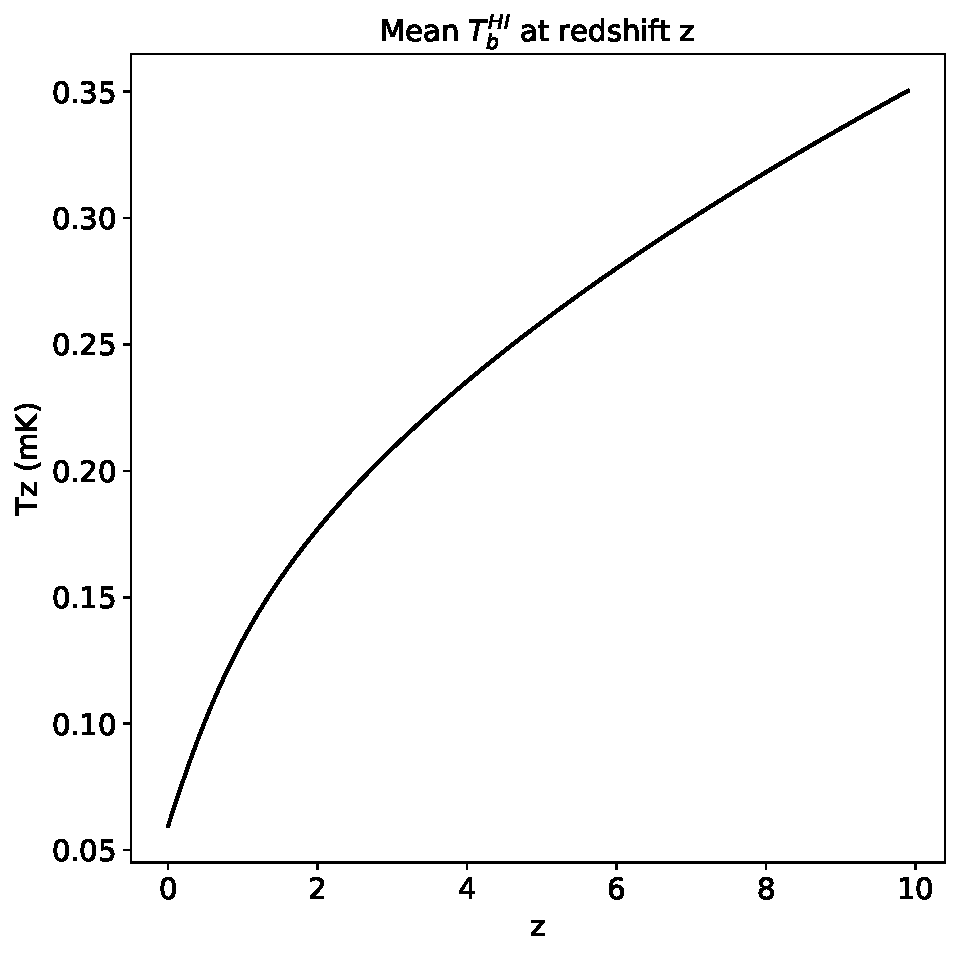
\includegraphics[width=0.7\textwidth]{variation-of-tz-with-z}
	\caption{Variation of $ HI $} brightness temperature with redshift. 
	\label{fig:tz-vs-z}
\end{figure}
Here and in Eq. 20 of P2014 I have taken
\begin{align}
E(z) &= \frac{H(z)}{H_0}\\
&= \sqrt{\Omega_{m_0} (1 + z)^3 + \Omega_{l}}.
\end{align}

\subsection{Matter power spectrum}
I have used the following code to obtain the matter power spectrum using Python CAMB.
\begin{lstlisting}[language=python]
pars = model.CAMBparams(NonLinear = 0, WantTransfer = True, H0 = 100 * h, omch2 = omegach2, ombh2 = omegabh2, YHe = YHe)
pars.DarkEnergy.set_params(w = -1)
pars.set_for_lmax(lmax = l_ul)
pars.InitPower.set_params(ns = ns, As = As)
#results = camb.get_background(pars)
results = camb.get_results(pars)
k = np.linspace(10**(-5), k_max(l_ul, z_s) ,1000)
PK = get_matter_power_interpolator(pars, nonlinear=False, kmax = np.max(k), k_hunit = False, hubble_units = False)
\end{lstlisting}

Some of the important parameters are:
\begin{itemize}
	\item \verb|NonLinear = 0|: Out of the four options available in CAMB for choosing the type of power spectrum, \verb|0| gives linear power spectrum with $ \sigma_8 \sim 0.8$ (so the normalization is correct), \verb|1| gives ``Non-linear Matter Power (HALOFIT)" and the other two have CMB in their name so we don't care. The \verb|nonlinear = False| also specifies that we wanr to generate a linear power spectrum. Before the thesis submission we were using \verb|NonLinear = 1| and \verb|nonlinear = True|, and that's why our convergence angular power spectrum was not matching with that of P2014. 
	\item \verb|k_unit = False| and \verb|hubble_units = False|: Read \verb|k| in Mpc units and output the power spectrum in Mpc units. \verb|True| will enable Mpc/h units.
	\item \verb|WantTransfer = True|: I need to find out what this option does, and if I can drop it. I am using this flag since the beginning.
	\item \verb|results = camb.get_background(pars)| and \verb|results = camb.get_results(pars)|: I am not sure what's the difference between the two; both work. I was using \verb|get_background| since the beginning because it is used in \href{https://camb.readthedocs.io/en/latest/CAMBdemo.html}{this CAMB demo}. I switched to \verb|get_results| because it can be used to find $\sigma_8$ by doing \verb|results.get_sigma8()| after we have defined what \verb|results| is as shown in the code.
	\item \verb|l_ul|: It is the upper limit in $ \int d^2l $ integrals in the lensing noise reconsruction expression (Eq. 14 of P2014). It is different from $ l_{max} $ defined in P2014 as the highest multipole visible to the instrument ($ l_{max}  = 19900 $ in P2014). The integrals, I think, should ideally go upto $ l = \infty $, so I usually take \verb|l_ul = 70000| or higher. We need to take such large number because we have 21-cm power spectrum terms in the noise expression. I think that if we take a smaller value for \verb|set_for_lmax| then the power spectrum would not be correct for large \verb|l| values of the integral.
\end{itemize}
Figure \ref{fig:matpowspec} shows the plot of matter power spectrum $ P_\delta(k) $ as a function of $ k $.
\begin{figure}
	\centering
	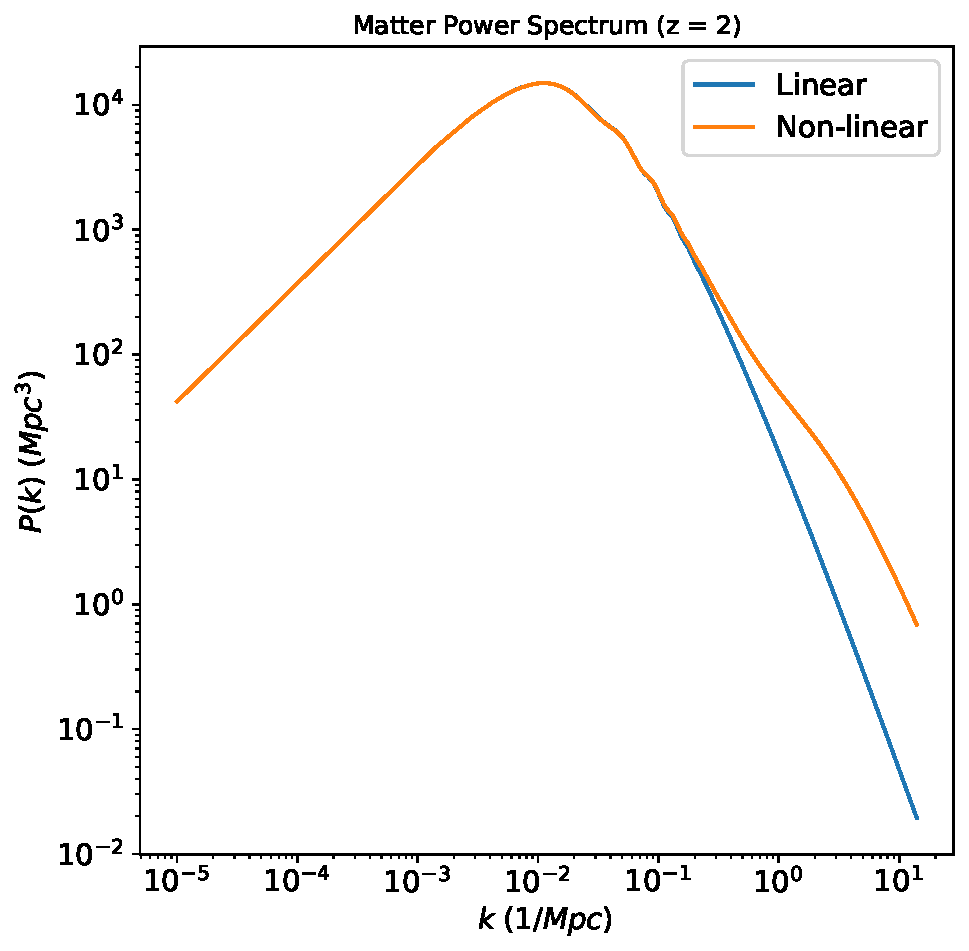
\includegraphics[width=0.5\textwidth]{matpowspec_2}
	\caption{A comparison of the linear and non-linear power spectrum. The linear power spectrum has been used in P2014.}
	\label{fig:matpowspec}
\end{figure}


\subsection{Power spectrum of 21-cm line}
Defining the 21-cm power spectrum using Eq. 2 of P2014 as 
\begin{align}
P_{\Delta T_b}(k) = [\bar{T}(z)]^2 (1 + f\mu_k^2)P_\delta(k),
\end{align}
where $ P_\delta(k) $ is the underlying (dark) matter power spectrum, $ f = \frac{d\;ln\; D}{ln\;a}$, $ D $ is the linear growth rate and $ \mu_k$ is the cosine of the angle between wavevector $ \textbf{k} $ and the line of sight $ \hat{z} $, and $ a $ is the scale factor $ (1 + z)^{-1} $.


I have ignored $ (1 + f\mu_k^2) $ in my calculations. The resulting 21-cm power spectrum is shown in Figure \ref{fig:21cm-powspec}

\begin{figure}
	\centering
	\begin{subfigure}{0.49\textwidth}
		\centering
		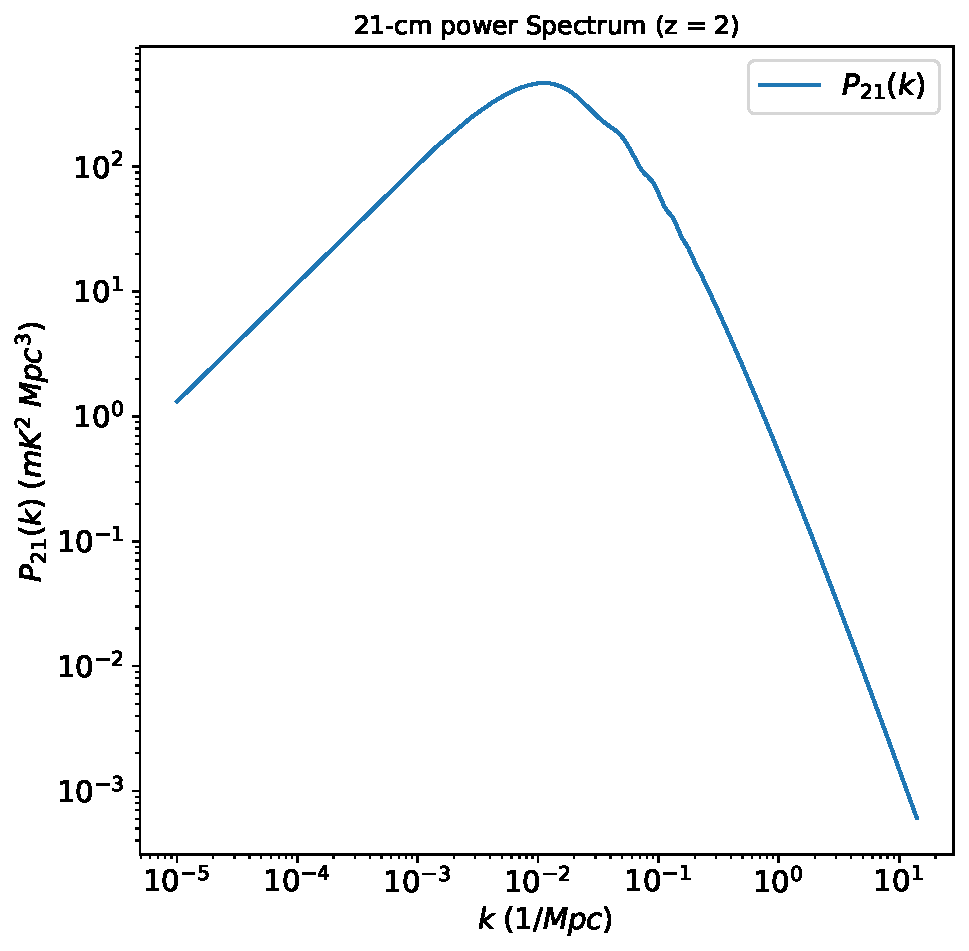
\includegraphics[width=\textwidth]{21cm-powspec_2}
		\caption{}
		\label{fig:21cm-powspec}
	\end{subfigure}
	\begin{subfigure}{0.49\textwidth}
		\centering
		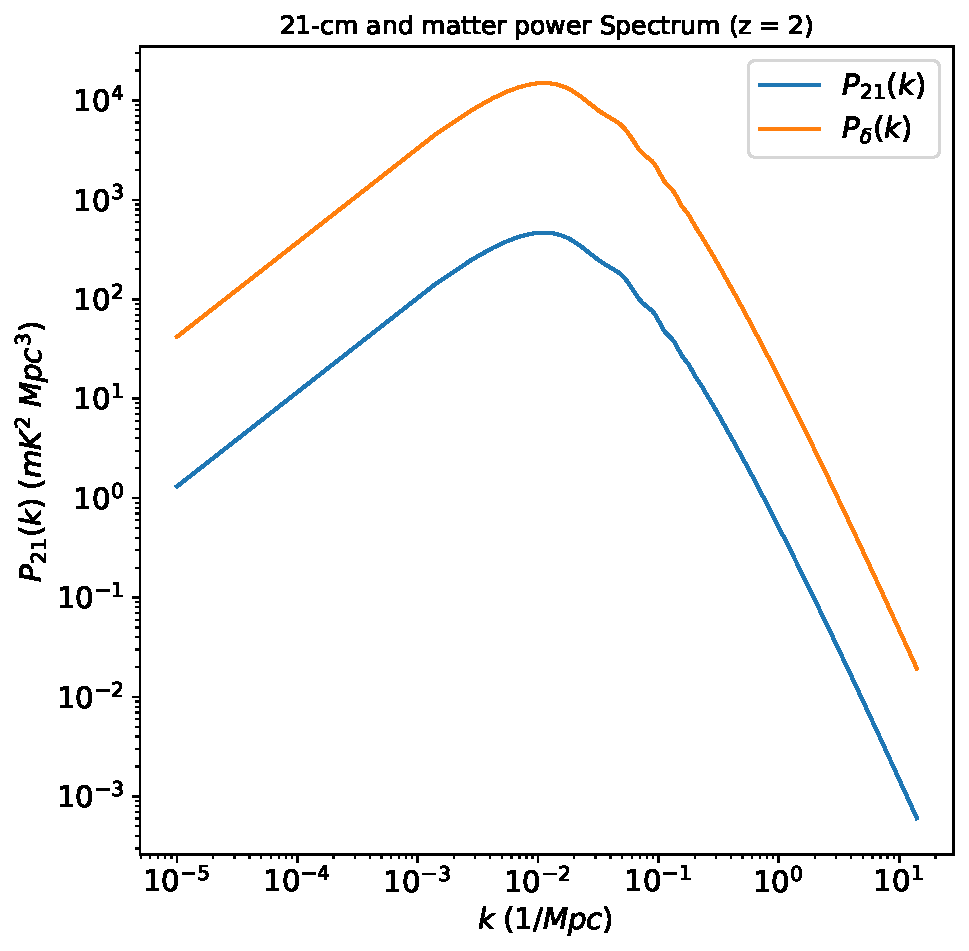
\includegraphics[width=\textwidth]{21cm-matter-powspec_2}
		\caption{}
		\label{fig:21cm-matter-powspec}
	\end{subfigure}
	\caption{(a) 21-cm power spectrum; (b) Comparison of 21-cm power spectrum with matter power spectrum}
\end{figure}


\subsection{Signam-to-noise ratio}
\subsubsection{Signal}
Prior to the thesis submission I hadn't really figured out how we are choosing our signal. I think I have now understood the concept of signal and noise in the context of lensing reconstruction. It's the following.

\begin{figure}[tbp]
	\centering
	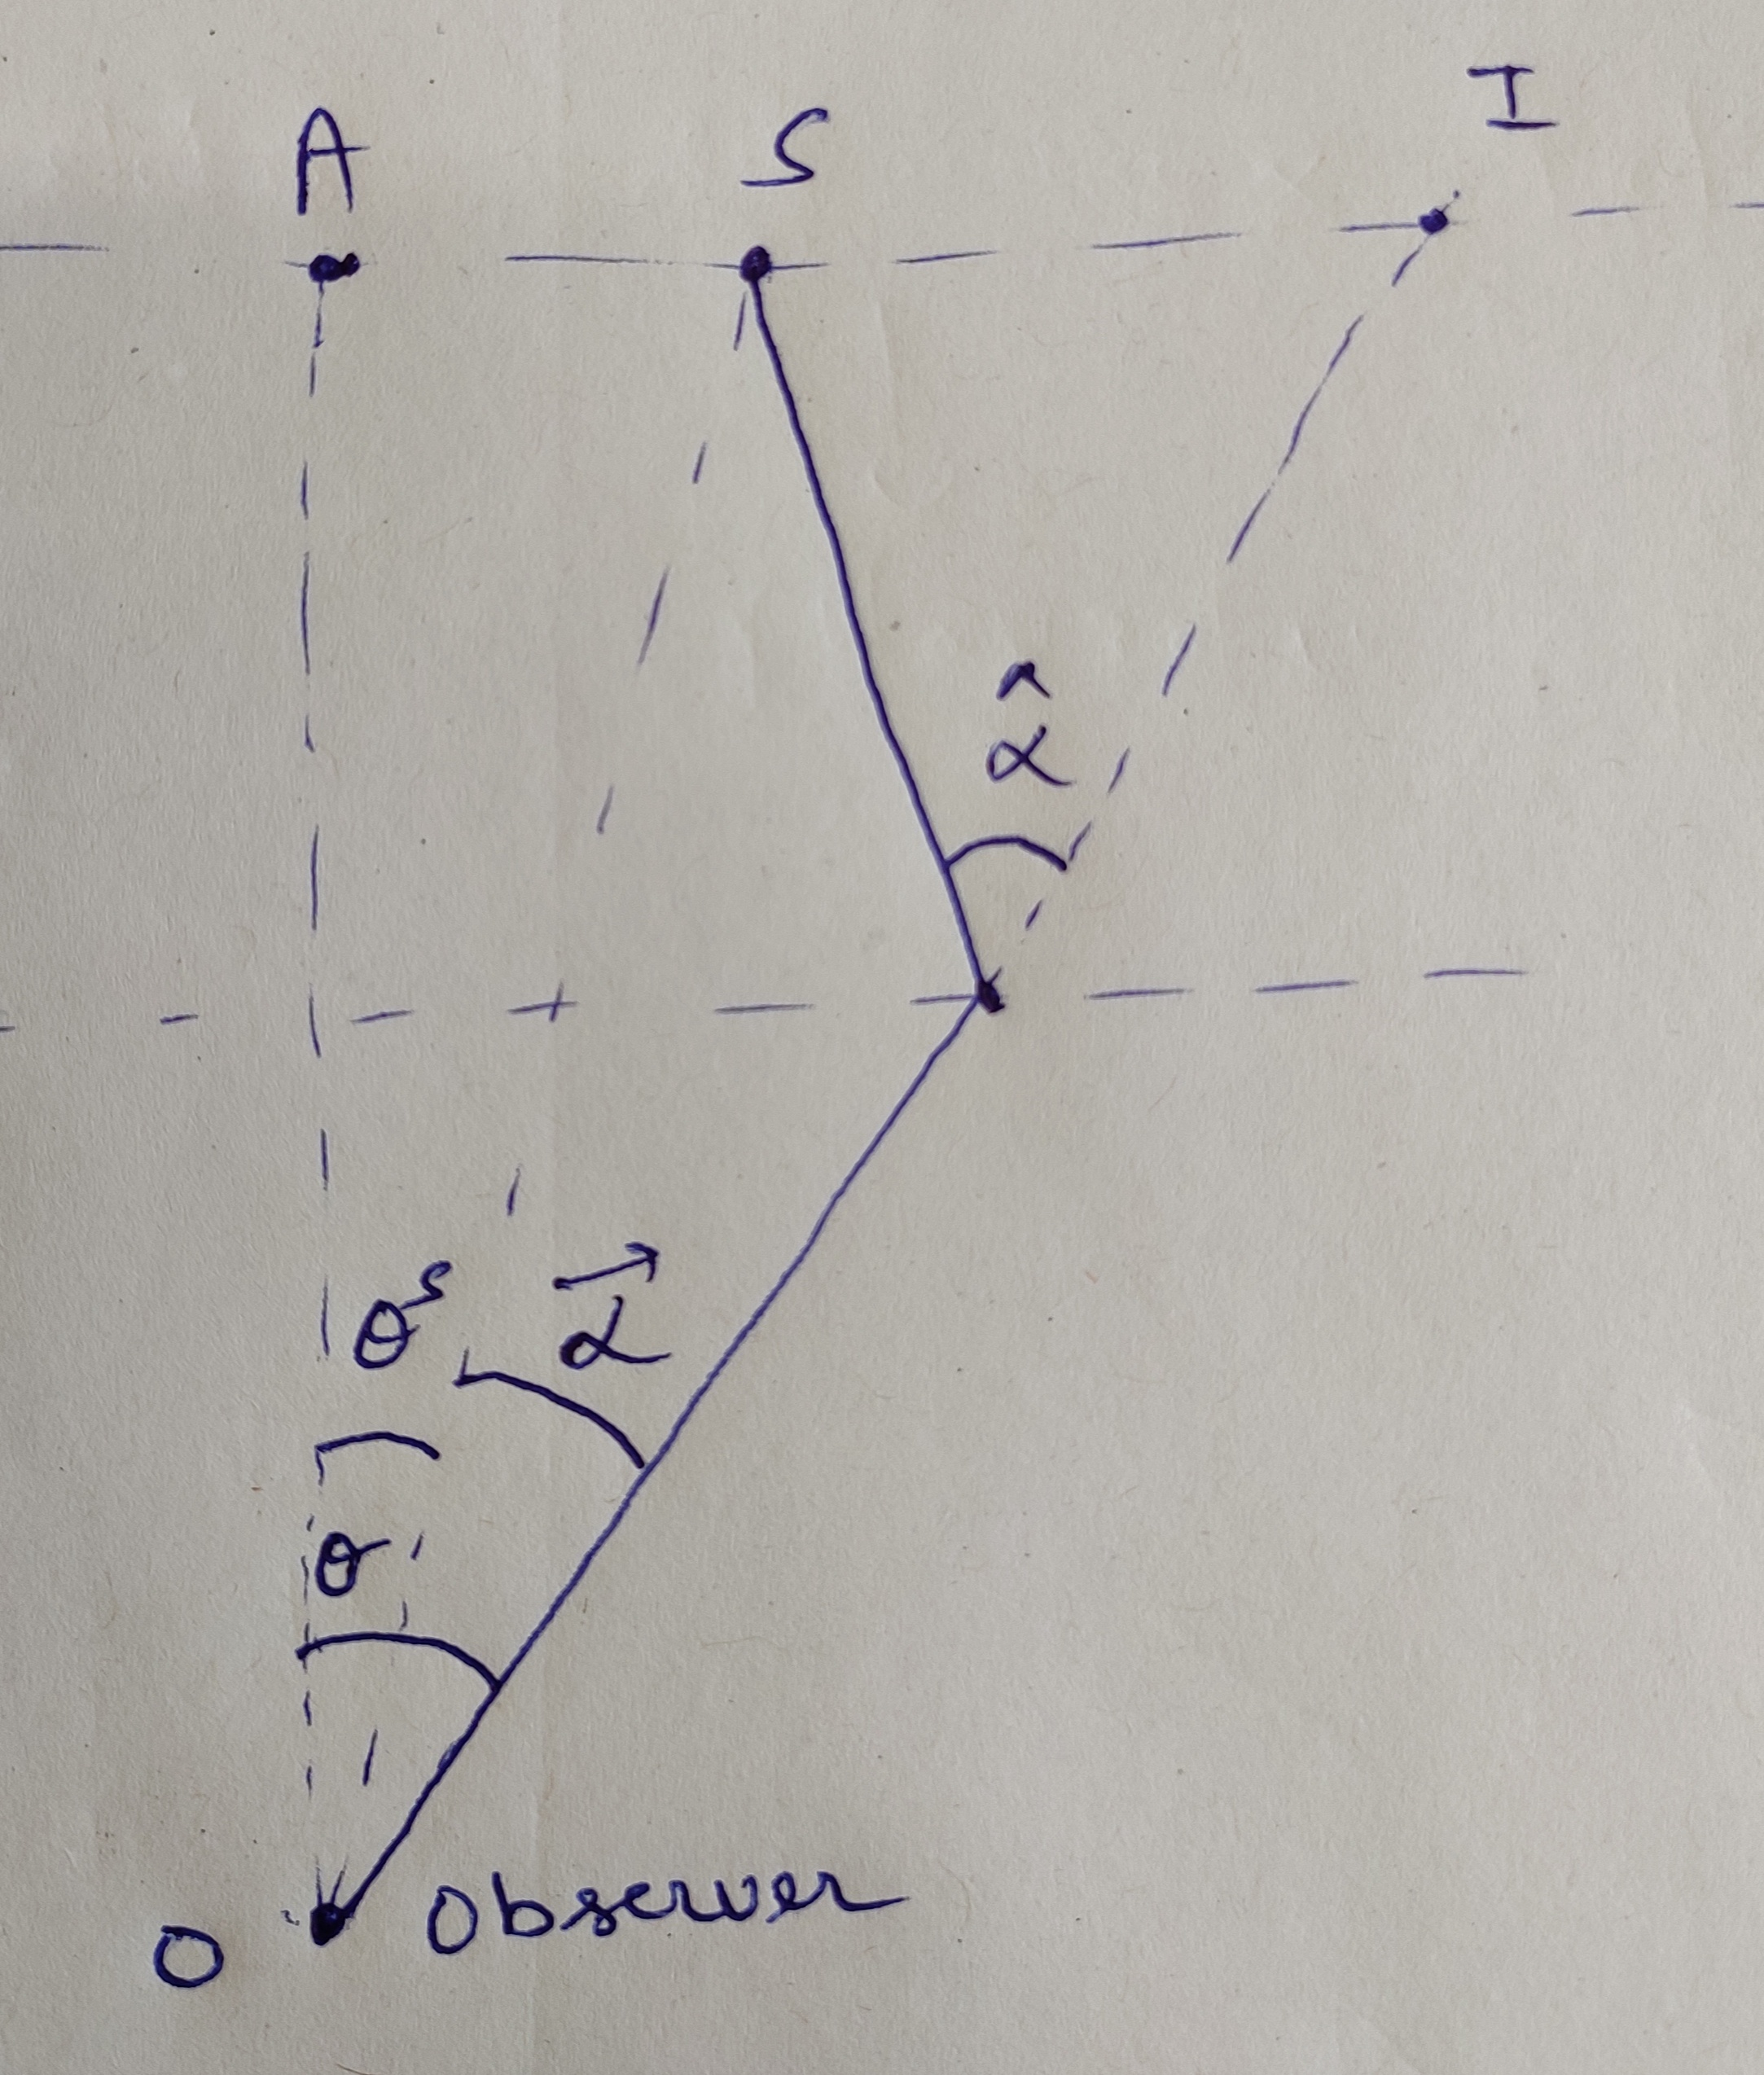
\includegraphics[width = 0.5\textwidth]{lensing_schematic}
	\caption{Schematic of a typical lensing setup. Only one lensing plane is shown for simplicity. Practically, the volume between the observer and the source can be thought of as a stack of many such planes of a certain thickness depending on the bin size we choose.}
	\label{fig:lensing_schematic}
\end{figure}

Figure \ref{fig:lensing_schematic} shows a typical lensing setup. The source is located at a transverse comoving distance \footnote{As per the definition given in Hogg 2006.} $ \chi $ away from the observer. The vector sign in $ \chi^{\vec{\theta}} $ signifies that there are two components of the transverse distance $ \chi^{\vec{\theta}} $ in the source plane -- one in the plane of the paper and the other perpendicular to it. Here, $ \hat{\alpha} $ is called deflection angle and $ \vec{\alpha} $ is called reduced deflection angle. We'll just need $ \vec{\alpha} $ to understand our signal.

Knowledge of $ \vec{\alpha} $ gives the observer the ability to map the images to the source. In other words, the observer reverses the lensing to obtain an unlensed distribution of sources. If we solve the  geodesic equation for the above set up, assuming perturbed FLRW metric, we get

\begin{align}
\vec{\alpha} =  \vec{\bigtriangledown}_{\theta}  \int_{0}^{\chi_s} d\chi^{\prime} \frac{2}{c^2}\Phi(\theta, \chi') \left(\frac{\chi_s - \chi^{\prime}}{\chi'  \chi_s}\right)  = \vec{\bigtriangledown}_{\theta} \psi, \label{eq:deflection_angle}
\end{align}
where $ \chi' $ represents the position of a particular lensing plane relative to the observer, $\Phi$ is the actual gravitational potential due to the mass distribution, and $\psi$ is called lensing potential.

But the problem is that we don't know $ \vec{\alpha} $ for any distribution. CONCERTO is going to record the mass distribution and shape features in its data and we can't find $ \vec{\alpha} $ from that data directly. So we need to relate $ \vec{\alpha} $ to another quantity that can be computed from the data.

Figure \ref{fig:lensing_schematic} gives
\begin{align}
\theta - \theta_s =  \vec{\alpha}
\end{align}
The following Jacobi matrix then gives the map to go from the source to the image. It basically tells us about the transformations by which the image differs from the shape of source.


\begin{align}
\mathcal{A}_{ij}(\chi_S, \theta) &\equiv \frac{\partial\theta_S^i}{\partial\theta^j} \\ 
&= \delta_{ij} - \psi,_{ij} \\
\implies
\mathcal{A} &= \underbrace{(1-\kappa) 
	\begin{pmatrix}
	1 & 0 \\
	0 & 1 \\
	\end{pmatrix}}_{isotropic}
+
\underbrace{
	\begin{pmatrix}
	- \gamma_1 & -\gamma_{2} \\
	-\gamma_{2} & \gamma_1 \\
	\end{pmatrix} 
}_{anisotropic} \label{eq:jacobi}
\end{align}

Here $\gamma_i$ are the components of shear and $ \kappa $ is convergence. Since we are dealing with cosmological weak lensing, we ignore the contribution from shear and take the isotropic term only. I am sure there's a better explanation for this, like convergence and shear are almost the same for weak lensing, but I am not going into that for now.

\paragraph{Question} When we say that we using taking convergence power spectrum 
in our calculations, does it mean that we are ignoring shear in the sense that it's not even there? Or does it mean that we are not considering the effect of shear on the map but it's there, and we are just looking at the effect of convergence?

\begin{figure}[tbp]
	\centering
	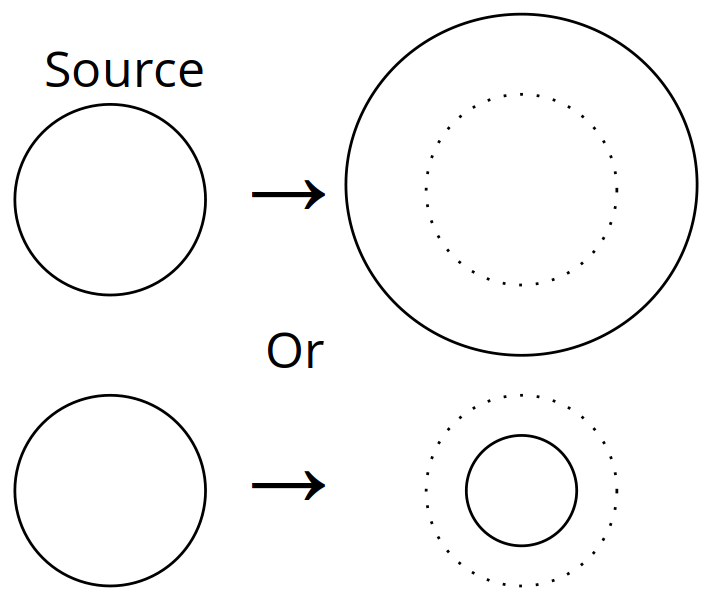
\includegraphics[width=0.5\textwidth]{convergence}
	\caption{Effect of convergence -- magnification for $ \kappa < 1 $ and demagnification for $ \kappa > 1$.}
	\label{fig:convergence}
\end{figure}

Figure \ref{fig:convergence} shows the effect of convergence for positive and negative values of $ \kappa $ in Eq. \eqref{eq:jacobi}. From this figure we see that convergence is a quantity that can be measured from the intensity mapping data (more on this later). Therefore, if we can relate $ \alpha $  with $ \kappa $ then the statistics of $\kappa$ will also be applicable to $ \alpha $.
%Let's assume that we are looking at one slice of the 3D volume that CONCERTO scan. In that sheet, on average, the size of the "structural features" is going to have some distribution

$\kappa$ is defined as 
\begin{align}
\kappa(\theta, \chi) = \frac{1}{2} \vec{\bigtriangledown}_\theta \cdot \vec{\alpha}(\theta, \chi).
\end{align}
Using this realation, we have connected a quantity $\vec{\alpha}$, which couldn't be computed from the data, with a quantity that can be computed via different statistical methods.

The quantity that we have chosen to compute is the power spectrum $ P^\kappa(k) $ of convergence, which is just the two-point correlation function of $\kappa$ in Fourier space. Assuming that $ \vec{l} $ is the Fourier conjugate to position $ \vec{\theta} $, we can write the angular power spectrum of the two quantities as 
\begin{align}
C^{\kappa\kappa}(L) &= \frac{1}{4}L(L+1) C^{\alpha\alpha}(L),\\
\implies C^{\alpha\alpha}(L) &= \frac{4}{L(L+1)} C^{\kappa\kappa}(L) \label{eq:disp_field_pow_spec}
\end{align}
where $ L $ is the observed Fourier mode. 

\paragraph{Error in thesis}Figure \eqref{eq:disp_field_pow_spec} is the reason for why we have $ 4/L(L + 1) $ in equation 20 of P2014. 

Eq. \eqref{eq:disp_field_pow_spec} gives us the statistic we wanted. We can now compute the displacement angle power spectrum from CONCERTO's data indirectly using convergence $\kappa$. So the final expression of our signa (in Pourtsidou's notation) is 
\begin{align}
C^{\alpha\alpha}(L) \equiv C^{\delta\theta\delta\theta}(L) = \frac{9 H_0^4 \Omega_{m0}^2}{L(L+1)c^4}  \int_0^{\chi_s} d\chi' \left[ \frac{(\chi_s - \chi')}{\chi_s} \frac{1}{a} \right]^2 P_\delta\left( \frac{L}{\chi'}\right).\label{eq:signal}
\end{align}
%What I submitted in the thesis is $ C^{\kappa\kappa} $. That's wrong because I did not make the corresponding changes to the lensing estimator and noise expression, and that messed up the units. The signal (convergence power spectrum) was in dimensionless units and the noise had dimensions of $ energy/c^2 $ (Eq. \eqref{eq:deflection_angle}).
Figure \ref{fig:signal} shows the plot of this expression. Our plot (signal only) now matches with that of P2014. Earlier we were using non-linear power spectrum and there was a lot of confusion about the units. Everywhere in P2014 they have used  $ Mpc/h $ units so I was expecting the same units in the plot. We were also under the impression that they have used non-linear power spectrum. Overall there were these four free variables (k units, P(k) units, linear, and non-linear) that I was trying to mix and match to see what combination worked. In the end it turned out that they have used the linear power spectrum with $ Mpc $ units.
\begin{figure}[tbp]
	\centering
	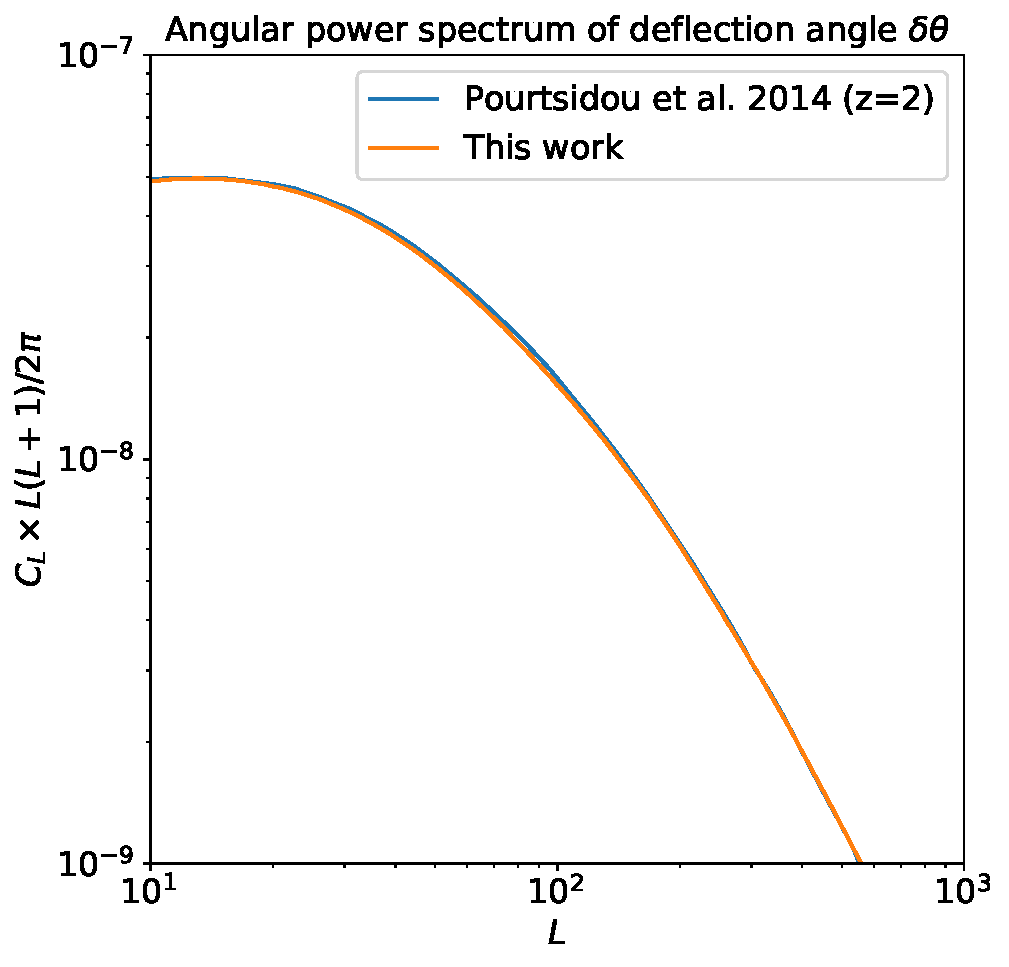
\includegraphics[width=0.5\textwidth]{c_l_z_2_lmax_50000_j_max_1}
	\caption{Our signal now matches with that of P2014.}
	\label{fig:signal}
\end{figure}


\subsubsection{Noise}
Just like we have found a quantity $ \kappa $ to indirectly measure the deflection angle power spectru, we also need to find the noise in the measurement of $ \vec{\alpha} $. In Eq, \eqref{eq:lensing_potential_estimator_form} we saw that $ \Psi \equiv \mathrm{lensing\;potential}$ is a natural choice for an estimator. So in Eq. \eqref{eq:lensing_potential_reconsruction_noise} we found the lensing reconstruction noise corresponding to the lensing potential measurement. But as we just discussed, we are measuring the deflection angle power spectrum, so we need to convert that noise accordingly.

The lensing potential $\psi$ and the deflection angle $ \vec{\alpha} $ are related as
\begin{align}
\vec{\alpha} = \vec{\bigtriangledown_\theta}\psi,
\end{align}
and the definition of lensing reconstruction noise ($ N[L] $) is
\begin{align}
\langle \hat{\tilde{\Psi}}(L)\hat{\tilde{\Psi}}(L') \rangle= 2\pi\delta(L - L') N^\psi(L),
\end{align}
therefore, using the relation between $ \vec{\alpha} $ and $\psi$ we write the lensing deflection angle reconstruction noise as
\begin{align}
N^{\delta\theta}(L) = L^2 N^\psi(L).\label{eq:general_displacement_field_reconstruction_noise}
\end{align}
In this equation we have indirectly found the noise in the measurement of displacement field power spectrum through the noise in the lensing potential measurement. This is a general result.

\subsubsection{Error bars}
The error in measurement of the deflection angle power spectrum is given by 
\begin{align}
\Delta C^{\delta\theta\delta\theta} = \sqrt{\frac{2}{(2L+1) \Delta L f_{sky}}}(C^{\delta\theta \delta \theta}(L) + N^{\delta\theta}(L)).
\end{align}
\paragraph{Error in thesis}
As I mentioned before Eq. \eqref{eq:signal}, I took $ C^{\kappa\kappa}(L) $ in place of $ C^{\delta\theta\delta\theta}(L) $.


\subsubsection{Gaussian noise}
We have derived the expression of $ N^\psi(L) $ for Gaussian matter distribution in equation \eqref{eq:general_displacement_field_reconstruction_noise}. Using that, we find the reconstruction noise for corresponding to the displacement angle power spectrum to be
\begin{align}
N^{\delta\theta} &= \frac{L^2}{\int \frac{d^2 l}{(2\pi)^2} \sum_{j} \frac{[C_{l,j} \L\cdot \l +
		C_{L-l,j} \L\cdot (\L-\l)]^2}{2C^{tot}_{l,j}C^{tot}_{L-l,j}} }
\end{align}
where $ C_{l, j} $ is the discretized 21-cm power spectrum defined as 
\begin{align}
C_{l,j} = \frac{P(\sqrt{(l/\chi^2) + (2\pi j / \mathcal{L})})}{\chi^2\mathcal{L}}
\end{align}

\subsubsection{Instrumental Noise}
\begin{align}
C_l^N = \frac{(2\pi)^3 T_{sys}^2}{B t_{obs}f_{cover}^2 l_{max}(\nu)^2 }
\end{align}

\subsubsection{Gaussian + Poisson noise}

\paragraph{Mass moments and number density of galaxies}
The number density of galaxies in the mass range $ dM $ is given by Schechter function
\begin{align}
\frac{dn}{dM}dM = \phi^\star \left(\frac{M}{M^\star}\right)^\alpha exp \left[\frac{-M}{M}\right] \frac{dM}{M^\star}
\end{align}
where $\alpha$ is the slope, $ M^\star $ is characteristic mass and $\phi^\star$ is normalization.

Using this we calculate the mass density of HI sources as
\begin{align}
\rho_{HI}  &= \phi^{\star}M^\star \int \left(\frac{M}{M^\star}\right)^{\alpha + 1} exp\left[ -\frac{M}{M^\star} \right]\frac{dM}{M^\star}\\
&= \phi^\star M^\star \Gamma(\alpha + 2)
\end{align}
where $ \Gamma $ denotes the Gamma function.

\paragraph{Average number density of galaxies} The given expression of Schechter function has a normalization constant. So is
\begin{align}
\int \frac{dn}{dM}dM = 1?
\end{align}

If not, then is
\begin{align}
\bar{\eta} &= \int \frac{dn}{dM}dM\\
&= \int \phi^\star x^\alpha e^{-\alpha} dx \\
&= \int \phi^\star x^{(\alpha + 1) - 1} e^{-\alpha} dx \\
&= \phi^\star\Gamma(\alpha + 1)
\end{align}

Here the integral blows up for $ \alpha < -1 $ but we still went ahead and wrote the Gamma function. 
Here for $ \alpha = -1.3 $ in our case, the argument of $\Gamma$ is negative. For negative non-integer values, the Gamma function is defined as
\begin{align}
\Gamma(1+x) = \frac{1}{1+x}\Gamma(2 + x),
\end{align}
where $ x < 1$. Now we can calculate $\bar{\eta}$ as

\begin{align}
\bar{\eta}  &= \phi^\star \frac{\Gamma(2 + \alpha)}{1 + \alpha}\\
&= -4.326
\end{align} 
for $ \alpha  = -1.3$.

\paragraph{Mass moments}
Defining the mass moment as
\begin{align}
\langle M \rangle &= \frac{\Phi^\star M^\star \int  x^{\alpha + 1} e^{-x}dx}{\bar{\eta}}\\
&= \frac{\phi^\star M^\star \Gamma[\alpha + 2]}{\bar{\eta}}
\end{align}
Therefore the $ n^{th} $ moment is
\begin{align}
\langle M^n \rangle = \frac{\phi^\star {M^\star}^n \Gamma(\alpha + n + 1)}{\bar{\eta}}
\end{align}
Here if $\bar{\eta}$ is negative then all the mass moments will be negative. But these are physical quantities. They can not have negative values.

\begin{figure}
	\centering
	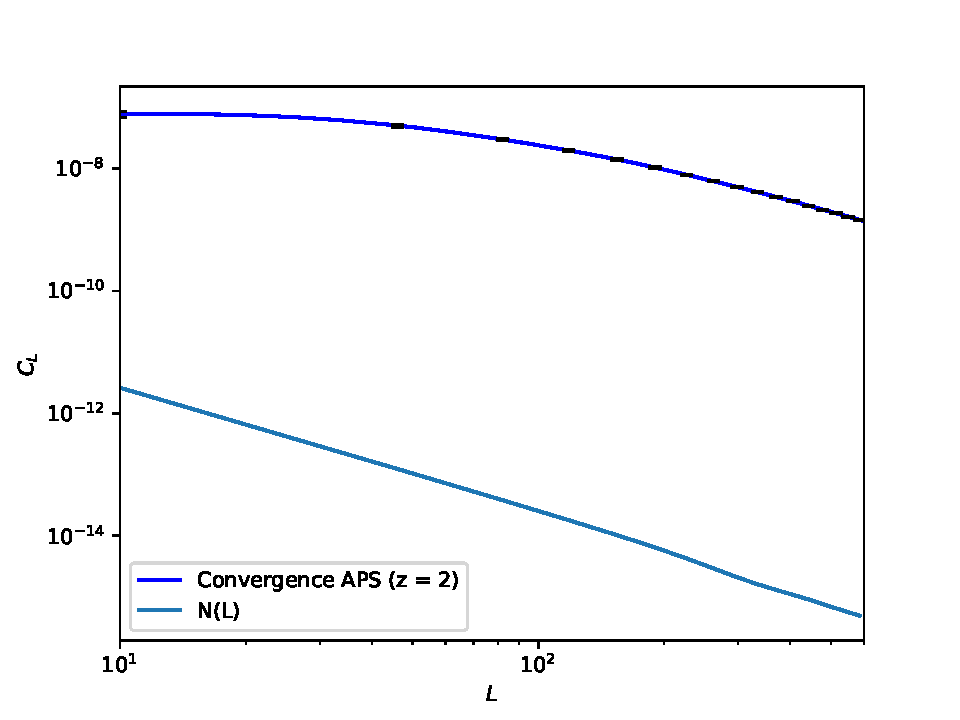
\includegraphics[width=0.7\textwidth]{full_plot_j_max_1_lmax_1000}
\end{figure}


\section{Figure 3 and 5 in Alkistis's notes -- 21-alk.pdf}
\subsection{Figure 3}
\subsubsection{Signal}
To plot the signal we use Eq. \ref{eq:signal} with the parameters taken from ZZ2006.

\paragraph{Parameters}
Parameters taken from ZZ2006
\begin{align}
h & = 0.7 \\
H_0 &= \frac{100\;h\,km}{sec\;Mpc}\\
\Omega_{m_0} &= 0.3 \\
\Omega_{b} &= 0.04 \\
\Omega_{c} &= \sqrt{\Omega_{m_0}^2 - \Omega_{c}^2}\\
\Omega_{l} &= 0.7\\
n_s &= 1\\
\sigma_8 &= 0.9\\
\end{align}
Here $\sigma_8$ is mentioned just for reference. It is not used to calculate the signal.






\end{document}

%\section{Signal to noise ratio for $z_{source} = 2 $ and Gaussian distribution}
%
%%\subsection{21 cm brightness temperature}
%%\begin{eqnarray}
%%\bar{T}(z) = 180 \Omega_HI(z) h \frac{(1+z)^2}{E(z)} mk
%%\end{eqnarray}
%%where $ h = H_0/100kms^{-1}Mpc^{-1} $, $ E(z) = H(z)/H_0$ (I call it Hubble ratio) and $ \Omega_HI(z)  = 8\pi G \rho_{HI}(z) / (3H_0^2)$ is the average density at redshift z relative to the present day critical density. More on $ \Omega_HI $ later when we calculate the noise for Gaussian + Poisson case.
%
%\section{SNR for Gaussian + Poisson distribution}
%Eq. 17 of Pou. et al. 2014
%
%\begin{eqnarray}
%\frac{dn}{dM}dM = \phi^\star \left( \frac{M}{M^\star} \right)^\alpha exp\left[\frac{-M}{M^\star}\right]\frac{dM}{M^\star}
%\end{eqnarray}
%
%This is the number density of of galaxies in a mass range dM (Schechter fn.).
%\subsection{Average number density $\bar{\eta}$}
%Defined below equation 9 of Pou. et al. 2014.
%
%\textbf{Problem}\\
%$\bar{\eta}$
%\begin{eqnarray}
%\bar{\eta} = \int \frac{dn}{dM}dM = \phi^\star \Gamma(\alpha + 1)
%\end{eqnarray}
%Is this result valid? The integral does not become a Gamma function for negative $\alpha$. We get infinity if we compute this integral. 
%
%\textbf{$\Gamma(\-a)$ is valid through analytic continuation}\\
%\href{https://math.stackexchange.com/questions/2204020/definition-of-the-gamma-function-for-non-integer-negative-values}{Link}
%
%\begin{eqnarray}
%\Gamma(a) = \frac{1}{a} \Gamma(1 + a)
%\end{eqnarray}
%for $ a<0 $ and non-integer $ a $.
%
%
%This gives negative $\bar{\eta}$. ($\Gamma(0.7)>0$)
%
%\subsection{Mass moments}
%\begin{eqnarray}
%<M> &=& \frac{\phi^\star M^\star \Gamma(\alpha + 2)}{\phi^\star \Gamma(\alpha + 1)}\\
%<M^2> &=& \frac{ (M^\star)^2 \Gamma(\alpha + 3)}{ \Gamma(\alpha + 1)}\\
%<M^3> &=& \frac{ (M^\star)^3 \Gamma(\alpha + 4)}{ \Gamma(\alpha + 1)}\\
%<M^4> &=& \frac{ (M^\star)^4 \Gamma(\alpha + 5)}{ \Gamma(\alpha + 1)}
%\end{eqnarray}
%
